 \documentclass[../main.tex]{subfiles}

\begin{document}
\section{Theoretical Background} \label{sec:theory}

\subsection{Machine Learning} \label{ssec:machine_learning}

The terms machine mearning (ML) and artificial intelligence (AI) are often used interchangeably, and not well distinguished. Therefore, before going into detail about machine learning both terms and their relation are pointed out.
\newline

Depending on the field of research there exists multiple definition for the term \acs{ai}. In the following paragraphs some definitions are presented giving an insight into the wide range of possibilities and angles one can look at the topic.
Based on the simple question "What is \acs{ai}?" one possible answer is "It is the science and engineering of making intelligent machines, especially intelligent computer programs. It is related to the similar task of
using computers to understand human intelligence, but AI does not have to
confine itself to methods that are biologically observable." \cite{mccarthy_what_nodate}
\newline

A different angle is to categorize AI in terms of weak AI and strong AI \cite{kuhl_machine_2020}, or narrow AI and \ac{agi}. Weak refers to an AI which pretends to think, strong AI refers to a mind with mental states. Narrow AI exceeds humans in a specific limited area or task while AGI mimics and acts on the same level as a human mind but without consciousness \cite{kurzweil_singularity_2006}.
\newline

In context of computer science, \acs{ai} research and its potential applications can be categorized by two streams. The objective, thinking vs acting, and the type of decision making, humanly or rationally. This leads to a categorization of four research types \cite[p.~5]{russell_artificial_1995}, \cite{kuhl_machine_2020}.
\begin{itemize}
    \item Cognitive modeling or thinking humanly, the ultimate goal would be to develop a machine imitating a mind.
    \item Turing test, implies acting humanly or show human like intelligence when interacting with humans.
    \item Laws of thought refers to thinking rationally, not necessarily give the same results as a human would do.
    \item Rational agent stream can be explained as acting rationally and refers to autonomous and intelligence agent following an objective achieving the rationally best outcome.
\end{itemize}

Based on different definitions and categorization it becomes clear that AI covers a wide range of topics and is still inaccurately defined. When looking at machine learning (\acs{ml}) the research stream of "Rational Agent" within AI comes closest to ML which leads to the conclusion that ML is a branch of AI. Tom M. Mitchell states, that "Machine learning (ML) is the study of computer algorithms that can improve automatically through experience and by the use of data" \cite{mitchell_machine_1997}.
\newline

Generally speaking machine learning involves "learning" by using experience, past events or collected facts in form of data. Usually in machine learning inductive learning in which rules or pattern are identified, is followed by a deductive inference process during which those learned rules are applied to solve a concrete task. For traditional algorithms especially in context of computer science those rules are not inductively learned, but predefined following laws of nature or business objectives. Within Machine Learning there are multiple types of learning problems which can be categorized as follows \cite{brownlee_14_2019}:

\begin{itemize}
    \item \textbf{Supervised machine learning (\acs{sml})} includes a mapping in form of some input data $x \in X$ and corresponding target data $y \in Y$ for which a mapping function $g: X \rightarrow Y$ must be learned. This mapping function can be parameterized $y=g(x; \phi)$ for which a fixed set of parameters $\phi$ must be learned, or non-parameterized $y=g(x)$ which primarily depends on the size of data of $x$ \cite{bishop_pattern_2006}. Depending on the type target data $Y$ there are two main types supervised learning problems:
    \begin{itemize}
        \item \emph{Classification} tasks which involve the prediction of concrete class labels or
        \item \emph{Regression} tasks that involve the prediction of a numerical value
    \end{itemize}

    \item \textbf{Unsupervised machine learning (\acs{uml})} describes methods which learn relationship within data $x\in X$ without any explicit given target data $y \in Y$. There is no "supervision" for the model during learning. Typical tasks are to find the "best" representation which usually is a simpler or more accessible version of $x$ while still preserving relevant information \cite{Goodfellow-et-al-2016}. Problems solved are for example:
    \begin{itemize}
        \item \emph{Clustering} problems, which try to find a predefined number of groups within data belonging together.
        \item \emph{Density estimation} which learns and summarizes the distribution of data.
    \end{itemize}

    \item \textbf{Semi-supervised learning} is an approach which blurs supervised with unsupervised learning. For each input data $x_1, ... x_l \in X$ there exists target data $y_1, ..., y_l \in Y$. Additionally $x_{l+1},...x_n \in X$ exists without any corresponding target data and is referred to as  unlabeled data. One simple approach is self-learning. In self-learning one case is to learn from target data similar to supervised learning and afterwards predict $\hat{y_{l+1}},...\hat{y_n} \in Y$. Afterwards use the combined set of $x_1, ... x_l + x_{l+1},...x_n \in X$ with target data $y_1, ..., y_l + \hat{y_{l+1}},...\hat{y_n} \in Y$ including predicted target data, usually thresholded to only include quality prediction, to relearn a model\cite{ligthart_analyzing_2021}. Other prominent approaches include generative models, graph-based learning or co-training \cite{chapelle_semi-supervised_2006}.

    \item \textbf{Self-supervised learning} refers to reformulating an unsupervised learning problem such that a supervised learning method can be applied. In such a way it is possible to learn representations without direct target data $y \in Y$. Those learned representations can be used in a downstream task, one example is to fine tune those on actual target data, possible in a different data domain \cite{kolesnikov_revisiting_2019}. One simple but prominent example is an Autoencoder. Given input data $x \in X$ there exists a parameterized encoder function $u$ which is used to learn a latent or hidden representation $h=v(x; \phi_{enc})$. Using a parameterized decoder function $v$ such that one is able to reconstruct the original input data $x$ as close as possible using the hidden latent representation, here referred to as $x'=v(h;\phi_{dec})$. 
    
    The concept of encoder and decoder is an important concept within machine learning in general and for self-supervised learning in particular. Other prominent examples are generative adversarial networks (\acs{gan}) \cite{goodfellow_generative_2014} or variational autoencoder (\acs{vae}) \cite{kingma_auto-encoding_2014}.

    \item \textbf{Reinforcement learning (\acs{rl})}  describes algorithms which can interact with an environment by learning from provided feedback seeking to achieve a defined goal or maximize a reward. As the learning involves a feedback loop, potentially noisy and delayed, there is no fixed data which is learned on \cite{sutton_reinforcement_nodate}.
\end{itemize}

Within machine learning beside the categorization of the learning problem also the learning technique is important and can be distinguished. Some important ones are briefly presented as follows:

\begin{itemize}
    \item \textbf{Multitask learning} refers to the fact that a method can learn multiple tasks at once. Using the same input data $x \in X$ we have multiple target data $y_1 \in Y_1$, and $y_2 \in Y_2$ such that a function $f$ (parameterized or non-parameterized) can learn to infer both set of target data $y_1, y_2 = f(x)$. This is especially useful in scenarios where the number of labeled data for multiple targets is not the same \cite[p.~244]{Goodfellow-et-al-2016}.
    
    \item \textbf{Active learning} refers to strategies how to effectively use  human or other expert systems in a machine learning data preparation loop. Especially in SML at some point in time those data must be annotated or labeled. In practice this process is very resource intensive and often labeling all data is not possible. Therefore, the machine learning method as learner must be able ask queries if stuck. There exists multiple query strategy frameworks. One simple approach is to start learning on few labeled data and relabel those data or new input data for which the learner or machine learning model cannot give a confident target prediction. This is refereed to as uncertainty sampling. Other strategies include variance reduction, expected error reduction or the query-by-committee approach \cite{settles_active_2009}.
    
    \item \textbf{Transfer learning} uses an already trained model which learned to solve one particular task within one data domain as a starting point for a subsequent task. Such a model is also referred to as pretrained model. Starting from a pretrained model a potential different task in a different but usually related data domain can be learned. This process is also referred to as fine tuning. Prominent examples for transfer learning can be found within the computer vision (\acs{cv}) field or within the natural language processing (\acs{nlp}) research stream \cite{zhuang_comprehensive_2020}.

    \item \textbf{Ensemble learning} describes the usage of multiple methods or learner $f_1,...f_n$ which all are trained on the same input data $x \in X$ having target data $y \in Y$. An aggregation or voting function $g$ is using individual learners output to return the overall decision $\hat{y}=g(f_1(x),...f_n(x))$. The idea is that an ensemble of learner can overcome individual errors or problems. In many machine learning challenges and real world applications an ensemble of methods often achieves state of the art performance. Prominent examples of methods which are build around ensemble learning are random forests refer to section \ref{par:rf} or gradient boosting decision trees refer to \ref{par:gbdt}. Both are using an ensemble of decision trees but ensemble learning is also able to combine multiple different types of methods or architectures \cite{sagi_ensemble_2018}.
\end{itemize}

Within the ML field there exists many different algorithms and methods to achieve the goal of learning. In the following some examples are listed and in the following sub-chapters for this work most relevant ones are described in detail.

\begin{itemize}
    \item \emph{Linear Regression} (section \ref{par:linear_model})
    \item \emph{Neural network} (section \ref{par:mlp})
    \item \emph{k-nearest neighbors (\acs{knn})}
    \item \emph{Support vector machine (\acs{svm})}
    \item \emph{Decision tree} (section \ref{ssec:dt})
    \item \emph{Naive Bayes}
    \item \emph{Perceptron and multilayer perceptron (MLP)} (section \ref{par:mlp})
    \item \emph{Recurrent neural network (\acs{rnn})}
    \item \emph{...}
\end{itemize}

\subsubsection{Decision-Tree based Methods} \label{ssec:dt}

Decision trees (\acs{dt}) are simple models which work by partitioning the input data into regions. A DT involves the selection of the best feature such that the data or distribution can be divided into most homogeneous parts. This is an iterative process which builds up the complete tree starting from a root node, selecting intermediate nodes and ends with homogeneous leaf nodes \cite{kotsiantis_decision_2013}.

Consider a classification problem with input feature vector $\mathbf{x} = (x_1, ... x_m)$ and binary target $y \in {0, 1}$. The actual training data consists of multiple input vectors $S={\mathbf{x_1},...\mathbf{x_n}}$ with corresponding target data $T={y_1,...y_n}$. First we need to select an element $x_1,...x_m$ of the feature space by which the overall training data can be split such the split is most homogeneous. In a binary case this could be in $T_{split}={y\in T | y = 1}$. 

In a complex feature space finding the optimal element by which to partition data is critical. Therefore, a concrete criteria or method is necessary to determine the optimal split. Two prominent splitting criteria are information gain and Gini impurity:

\begin{itemize}
    \item \textbf{Information gain (\acs{ig})} is based on the concept of reduction of entropy. The idea is that larger information gain is based on a lower entropy and therefore a favored split. Consider a discrete random Variable $X={x_1,...x_n}$ with probability $P(x_1),...P(x_n)$ the entropy (Shannon) can be written down as follows:

    \begin{equation}    
        H(X) = -\sum_{i=1}^{n} P(x_i) \ log(P(x_i)) =  \sum_{i=1}^{n} P(x_i) \ I(x_i) = \mathbb{E}[-log(P(X)) = \mathbb{E}[I(X)]
    \end{equation}

    The term $I(X)$ or $-log(P(X)$ refers to the self-information of information context. For example a dice having only one value on all sides would have no entropy (0). This is also referred to as purity or no surprise within information theory framework.

    Information gain for a single subset or split can be described as the difference between, a prior entropy of the data and the entropy of the conditional data given a certain feature $x_a$:

    \begin{equation}
        IG(S, x_a) = H(S)-H(S|x_a)
    \end{equation}

    More generally defined for a given node $S_i$ the information gain is defined over its $k$ splits or child nodes $S_1, \ldots S_k$. $\frac{|S_j|}{|S|}$ denotes the number of elements in that split and is basically weighting the entropy:

    \begin{equation}
        IG = H(S,i) - \sum_{j=1}^{k} \frac{|S_j|}{|S|} H(S_j), 
    \end{equation}

    Lets consider a balanced binary classification task $T={0,1,0,1}$ for which we split the data perfectly into two homogeneous groups $T_1={0,0}$ and $T_2={1,1}$. The IG would be calculated by using a prior entropy minus the two groups entropy $IG=H(T)-1/2 * H(T_1)-1/2* H(T_2)=1$. For the other extreme ($T_1={0,1}$, $T_2={0,1}$) the information gain would be $IG=H(T)-1/2 * H(T_1)-1/2 * H(T_2)=0$. The later one would be considered an inferior split compared to the first split.

    \item \textbf{Gini impurity gain $g_G$}, is a concept using the Gini impurity ($I_G$) which is refereed to if an element from a set is randomly chosen and incorrectly labeled by randomly selecting a label from the distribution of labels. This can be defined as follows:

    \begin{equation}
        I_G(S)=1-\sum_{j=1}^{J}p_j(S)^2
    \end{equation}

    $J$ denotes the number of target classes while $p_j(S)$ describes the frequency of occurrence of one particular class within one set.
    Naturally it follows if all labels in a set fall within one class the $I_G$ would be 0. The $g_G$ is defined as given:
    
    \begin{equation}
        g_G(S) = I_G(S) - \sum_{j=1}^K \frac{|S_k|}{|S|} \cdot I_G(S_k)
    \end{equation}
    
    As an example consider the balanced binary classification tasks $T={0,1,0,1}$ with again two perfectly homogeneous groups $T_1={0,0}$ and $T_2={1,1}$. The Gini impurity gain would be calculated as $g_G(T)=1-1/2*I_G(T_1)-1/2*I_G(T_2)=1-1/2*0-1/2-0$ and considered perfect or pure.
\end{itemize}

To actually build up a decision tree multiple algorithms exist. One of the earliest one is ID3 (Iterative Dichotomiser 3) introduced in 1986 by Ross Quinlan \cite{quinlan_induction_1986}. ID3 supports categorical features and iterates over the available features in a greedy way using IG to identify the ideal splitting feature at each node. The successor to ID3 is C4.5 which supports also numerical features by dynamically partition a numerical feature into discrete set of intervals. An alternative algorithm is CART (Classification and Regression Trees) similar to C4.5 but directly supporting numerical features using a threshold to define splits \cite{noauthor_110_nodate}.

General advantages of decision trees are that they are relatively simple and easy to interpret. Disadvantages are that they tend to overfit the data and are sensibly to outliers and small changes in the data. Therefore usually decision trees are combined as an ensemble of trees and trained using methods like random forest (\acs{rf}) and gradient boosting decision tree (\acs{gbdt}).

\myparagraph{Random Forest} \label{par:rf}

Random forest (\acs{rf}) describe the usage of multiple decision trees as an ensemble. The bases for RF was first introduced in 1995 by Tin Kam Ho \cite{ho_random_1998} and refined in 2001 by Leo Breiman \cite{breiman_random_2001}. One of the main concept is called "bagging". For this concept two variants are used within RF.

\begin{itemize}
    \item \textbf{Bagging} describes the basic technique of bootstrapping or bootstrap aggregation. Consider dataset $S=(x_1,...x_n)$ with target data $T=(y_1,...y_n)$ we sample with replacement $K$ sub-datasets $S_k, T_k$ consisting of $m$ entries ($m<n$). For each of the sub-dataset a decision tree $f_k$ is created or trained in a SML typical setting $T_k=f_k(S_k)$. During inference unseen data $S'$ uses the overall result or prediction of the majority vote of the individual decision tree. This can be defined as follows:

    \begin{equation}
        \hat{T}=\frac{1}{K}\sum_{k=1}^{K}f_k(S')
    \end{equation}

    \item \textbf{Feature bagging}, similar to bootstrap aggregation using a random sample of individual entries within the data feature bagging refers to using a random sub-sample of features $a$ during the build up of the individual trees. For example in the binary classification case typically only $\sqrt{a}$ are considered to determine the best split.
\end{itemize}

In contrast to decision trees a RF is less likely to overfit due to bootstrap aggregation. Due to the complexity of many decision trees combined in an ensemble to interpret the results or prediction is more difficult.

\myparagraph{Gradient Boosting Decision Tree} \label{par:gbdt}

Beside bootstrap aggregation like in RF another possibility to build up trees is using a technique called gradient boosting (GB). 
Before defining GB formally consider the overall model $F$ which predicts values as $\hat{y}=F(x)$. To build up $F$ GB uses $M$ estimators which sequentially build up an ensemble which is used for the final prediction. Starting from an imperfect function $F_m$ which could be a constant function or the average function $\hat{y_i}=\bar{y}$ another more refined function or estimator $h_m$ is added.

\begin{equation}
    F_{m+1}(x)=F_m(x)+h_m(x)=y 
\end{equation}

This could be reformulated as

\begin{equation}
    h_m(x)=y-F_m(x)
\end{equation}

and describes that in GB $h_m$ is using the error or residual $y-F_m(x)$ as training data. In general boosting refers to the technique iteratively correct the error of the predecessor model. If $h_m$ is fitted on the gradient $g$ of a loss function $L$ such as

\begin{equation}
    g_m=\frac{\partial L(y, F_m(x))}{\partial F_m(x)}
\end{equation}

the algorithm is referred to as gradient boosting or gradient boosting machine \cite{friedman_greedy_2001}.

The general GB algorithm can be described as follows. Starting from a constant value function $F_0(x)$ using a differentiable loss function $L$ with data ${x_i, y_i}_{i=1}^{N}$ GB can be described as follows \cite{friedman_greedy_2001}:

\begin{equation}
    F_0(x)=\underset{p}{\mathrm{argmin}}\sum_{i=1}^{N}L(y_i,p) 
\end{equation}

For $1<=m<=M$ boost or improve the overall function model $F$ by first calculate the pseudo-residual of the $m-1$ improved model $F$:

\begin{equation}
    r_{im}=-\frac{\partial L(y_i,F_{m-1(x_i)})}{\partial F_{m-1}(x_i)}
\end{equation}

Fit a base or weak learner (e.g. a decision tree) $h_m$ using ${x_i, r_im}_{i=1}^{N}$ as training data. Afterwards approximate the optimal coefficient $p_m$ using line search:

\begin{equation}
    p_m=\underset{p}{\mathrm{argmin}}\sum_{i=1}^{N}L(y_i,F_{m-1}(x_i)+p h_m(x_i))
\end{equation}

Within each step boost the overall model 

\begin{equation} \label{eq:gb_update}
    F_m(x)=F_{m-1}(x)+p_mh_m(x)
\end{equation}

which results in the final output model $F_M$.

When using a decision tree as a base or weak learner there exists multiple different implementations. Those differ in the way the decision tree is fitted and the residual or gradients are used to build up the individual trees. For details refer to the most prominent implementations which are XGBoost \cite{chen_xgboost_2016}, LightGBM \cite{ke_lightgbm_2017} and CatBoost \cite{prokhorenkova_catboost_2019}.


\subsubsection{Deep Learning} \label{sssec:dl}

The bases for deep learning (\acs{dl}), using neural networks (\acs{nn}) and many of its fundamental concepts are around since decades. Due to the ever-increasing computational power, especially processing units performing exceptional well doing linear algebra (e.g., graphical processing units - GPU), the research field of neural networks reemerged as deep learning. The recently available computational power and break-through in research enabled neural networks with complex architectures with many billions of parameters and having multiple layers. Mainly the fact of having many layers within a NN lead to the term deep neural networks (\acs{dnn}) and deep learning. In the following the core concepts of NN and DL are presented roughly following terminology and structure of Klambauer et al. \cite{klambauer_notes_2019}.

\myparagraph{Linear Model} \label{par:linear_model}

A single output linear model describes a single output or target $y$ which can be described by a linear combination of up to $D$ features defined by input vector $\mathbf{x}$. This can be defined as:

\begin{equation} \label{eq:single_linear}
    y=\mathbf{w}^T\mathbf{x} + b
\end{equation}

$y \in \mathbb{R}$ refers to the output, $\mathbf{x}\in \mathbb{R}^D$ and $ \mathbf{w}\in \mathbb{R}^D$ are the coefficients or parameters. $b$ refers to the bias or error term, within linear models referred to as noise. Within a multi task linear model the output becomes $\mathbf{x}\in \mathbb{R}^K$, the parameters become the matrix $\mathbf{W} \in \mathbb{R}^{K \times D}$ and the bias is defined as $\mathbf{b}\in \mathbb{R}^K$. Combined this can be written as:

\begin{equation}
    \mathbf{y}=\mathbf{W}\mathbf{x} + \mathbf{b}
\end{equation}

For the single output linear model giving $N$ samples such that $\mathbf{y}\in \mathbb{R}^{N}$ and $\mathbf{X}\in \mathbb{R}^{N \times D}$ the task is to minimize the empirical error $R_{emp}(\mathbf{y}, \mathbf{X}, \mathbf{w}, b)$. This describes the usage of an objective or loss function $L$ on all available samples $N$ to find the optimal parameters $\mathbf{w}, b$ such that $R_{emp}$ becomes minimal. 

For linear models one objective could be the squared residuals $(\mathbf{y} - (\mathbf{w}^T\mathbf{X} + b))^2$. If summed up over all $N$ samples this is referred to as residual sum of squares (RSS). It follows that $R_{emp}$ for linear model using RSS can be defined as:

\begin{equation}
    R_{emp}(\mathbf{y}, \mathbf{X}, \mathbf{w}, b)=L(\mathbf{y}, \mathbf{X} | \mathbf{w}, b)=\frac{1}{2}(\mathbf{y}-(\mathbf{X}\mathbf{w}+b))^T(\mathbf{y}-(\mathbf{X}\mathbf{w}+b))
\end{equation}

To find the optional estimator $\hat{\mathbf{w}}, \hat{b}$ one needs to solve the following equation:

\begin{equation}
    \hat{\mathbf{w}}, \hat{b}=\underset{\mathbf{w}, b}{\arg\min}(L(\mathbf{y}, \mathbf{X} | \mathbf{w}, b))
\end{equation}

For a linear model there exists a closed solution using RSS as $L$ which results in the best unbiased estimator for $\hat{\mathbf{w}}, \hat{b}$ \cite[p.~146]{bishop_pattern_2006}. %TODO check reference

When the output is a binary classification the output becomes $y \in (-1,1)$. Such regression model is possible if a "sign" function or step function is applied to the output of a liner model and can be described as:

\begin{equation}
    y=sign(\mathbf{w}^T\mathbf{x})
\end{equation}

The sign function is thresholded around 0, meaning if the intermediate output $a$ within the linear transformation $a=\mathbf{w}^T\mathbf{x} \ge 0$ $y=1$ otherwise $y=-1$. This setup is also referred to as perceptron. For a perceptron there exists no closed form solution for the best estimator of parameters $\hat{\mathbf{w}}$. If data and classes are linear separable, a perceptron can be used and trained using a simple update rule based on the gradient w.r.t. $\mathbf{w}$. As the $sign$ function is non continuous the overall result is either true, separable or not separable. Updating using the gradient therefore in sequential manor will not converge in non-separable target data scenario.

\myparagraph{Logistic Regression} \label{par:logreg}

For non-linear scenarios the sigmoid function $\sigma$ can be used to approximate the $sign$ function in an probabilistic way. The output $y$ is within the interval $[0, 1]$ and describes the probability that $y=1$. $\sigma$ is defined as:

\begin{equation}
    \sigma(x)=\frac{1}{1+e^{-x}}
\end{equation}

\begin{figure}[H]
    \centering
    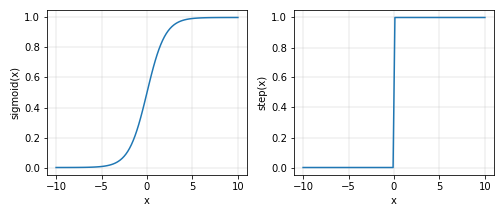
\includegraphics[width=0.8\textwidth]{sigmoid_step}
    \caption{$\sigma$ function on the right side as the approximation of an step function}
    \label{fig:sigmoid_step}
\end{figure}

When using $\sigma$ on the output of a single target linear model this can be described as a single linear neuron with $\sigma$ activation. In the context of neural networks and deep learning this is also referred to as an activation function. The linear neuron with $\sigma$ activation is defined as:

\begin{equation} \label{eq:logneuron}
    y=\sigma(\mathbf{w}^T\mathbf{x})
\end{equation}

Analog to linear regression the optimal parameters of the model $\mathbf{\hat{w}}$ (for simplicity the bias term $b$ is not included here) needs to be determined such that the $R_{emp}$ becomes minimal. As loss function $L$ for the $R_{emp}$ in the logistic regression setting the binary cross entropy is used and defined as follows:

\begin{equation} \label{eq:bce_loss}
    R_{emp}(y, \mathbf{x}, \mathbf{w})=L(y, \mathbf{x} | \mathbf{w}))=- \bigg( y\log\Big(\sigma(\mathbf{w}^T\mathbf{x})\Big) + (1-y) log \Big(1-\sigma(\mathbf{w}^T\mathbf{x})\Big)\bigg)
\end{equation}

There exists no closed form solution for the $\sigma$ function therefore an iterative approach using the first order gradient of the $L$ function w.r.t. $\mathbf{w}$ is used. First the gradient of $\sigma$ w.r.t. $\mathbf{w}$ is defined as:

\begin{equation}
    \frac{\partial \sigma(\mathbf{w}^T\mathbf{x})}{\partial \mathbf{w}} = \Big( \sigma(\mathbf{w}^T\mathbf{x})(1-\sigma(\mathbf{w}^T\mathbf{x})) \Big) \frac{\partial \mathbf{w}^T\mathbf{x}}{\mathbf{\partial w}}= \Big( \sigma(\mathbf{w}^T\mathbf{x})(1-\sigma(\mathbf{w}^T\mathbf{x})) \Big) \mathbf{x}
\end{equation}

Using $\frac{\partial \sigma(\mathbf{w}^T\mathbf{x})}{\partial \mathbf{w}}$ the gradient of the binary cross entropy loss function as defined in equation \ref{eq:bce_loss} w.r.t. to $\mathbf{w}$ is given as:

\begin{equation}
    \nabla_{\mathbf{w}} L(y, \mathbf{x} | \mathbf{w})) = \frac{\partial L(y, \mathbf{x} | \mathbf{w}))}{\partial \mathbf{w}} = (\sigma(\mathbf{w}^T\mathbf{x}) - y)\mathbf{x}
\end{equation}

Using the gradient $\nabla_{\mathbf{w}}$ the parameters are updated until convergence of the loss function $L$ or up to a defined maximum number of iterations $T$. This process is called gradient descent and given as:

\begin{equation}
    \mathbf{w^{t}} = \mathbf{w^{t-1}} - \eta\nabla_{\mathbf{w^{t-1}}}
\end{equation}

The term $\eta$ determines the size of the step which is taken into the direction of a local minima of the loss function $L$. This is refereed to as learning rate and a key concept within gradient descent and DL.
\newline

\myparagraph{Multilayer Perceptron} \label{par:mlp}

Even though within logistic regression a non-linear function $\sigma$ is used, some non-linear problems like the XOR problem can not be solved with just a single layer or transformation in the form of $y=f(\mathbf{w}^T\mathbf{x})$ with $f$ as an non linear activation function (e.g., $\sigma$) \cite{minsky_perceptrons_1969}.

When using multiple layers or transformations in which the output of one layer is the input of a subsequent one the XOR problem can be solved. The basic form of a multiplayer perceptron (MLP) using a $\sigma$ activation function is given as:

\begin{equation} \label{eq:mlp}
    y=\sigma(\mathbf{w}^T \sigma(\mathbf{W}\mathbf{x}))
\end{equation}

\begin{figure}[H]
    \centering
    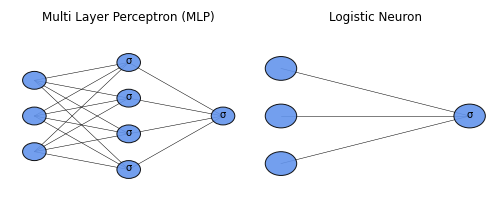
\includegraphics[width=0.8\textwidth]{mlp_logneuron}    
    \caption{Multilayer perceptron (MLP) sample with 2 layers on the left, single layer linear neuron sample with $\sigma$ activation (logistic neuron) on the right.}
    \label{fig:mlp_logneuron}
\end{figure}

Within figure \ref{fig:mlp_logneuron} an example MLP is shown with 2 layers. The middle layer is referred to as intermediate or hidden layer, in this example having 4 neurons. The principal architecture of any neural network is similar and only differs in the number of hidden layers, neurons, activation functions used and output activation. The term deep has no defined common meaning and only indicates a NN having multiple layers. This is also referred to as deep neural network (DNN). 
\newline

The components of any MLP or NN(DNN) can be summarized as follows:
\begin{itemize} 
    \item Having multiple layers ($1<=l<L$).
    \item Having multiple parameter sets in the form of $\mathbf{W}^l$ connecting layer $l-1$ with layer $l$.
    \item The size of each individual hidden layers $H$, referred to as nodes or neurons. This is also reflected in the dimension of the parameter matrix $\mathbf{W}^l\in\mathbb{R}^{H^l \times H^{l-1}}$. 
    \item A parameter set $\mathbf{W}^0\in{\mathbb{R}^{H^l \times D}}$ connecting the input data $x\in\mathbb{R}^D$ with the first hidden layer.
    \item A parameter set $\mathbf{W}^L\in{\mathbb{R}^{K \times H^{l-1}}}$ connecting the last hidden layer with the output data $y\in\mathbb{R}^K$.     
    \item A non-linear activation function $f$. The output is referred to as the activation of a layer $a^l$. The function $f$ is applied using the output of the linear transformation between the parameter set of the corresponding layer and the activation of the previous layers in form of $a^l=f(\mathbf{W}^l a+^{l-1})$.
    \item A bias term $\mathbf{b}\in\mathbb{R}^{H}$ which is added to the pre-activation $\mathbf{W}^l a^{l-1} + \mathbf{b}$. The term is optional and not further considered in the following equations.
    \item An output activation function $\tau$ depending on the task.
\end{itemize}

Defining the pre-activation $\mathbf{s}^l=\mathbf{W}^l \mathbf{a}^{l-1}$ the formal description of a MLP is given as follows, this is also referred to as the forward path:

\begin{equation}
    \mathbf{\hat{y}}
    =\tau(\mathbf{W^L(f(\mathbf{W^{L-1}(f(\mathbf{W^{L-2}(\dots f(W^0\mathbf{x}))}))}))}
    %=\tau(\mathbf{s}^L(f(\mathbf{s}^{L-1}(f(\mathbf{s}^{L-2}(\dots f(\mathbf{s}^0))}))}))}
\end{equation}

In figure \ref{fig:dnn} an schematic DNN is shown. The edges represent individual parameters in the parameter matrix $\mathbf{W}^l$. This concrete example having $L=4$, input dimension $D=3$, with overall 605 parameters. 

\begin{figure}[H]
    \centering
    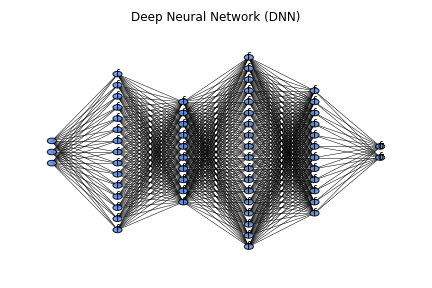
\includegraphics[width=0.8\textwidth]{dnn}    
    \caption{Multilayer perceptron (MLP) having many layers, referred to as neural network (NN) or deep neural network (DNN)}
    \label{fig:dnn}
\end{figure}

Analog to logistic regression, refer to section \ref{par:logreg}, a DNN is trained and optimized using gradient descent. Therefore using a differentiable loss function $L$ the gradient w.r.t. each individual parameter set $\mathbf{W}^l$ is calculated.

For the parameters set $\mathbf{W}^L$ connecting the last hidden layer with the target data $y$ this is defined as:

\begin{equation}
    \frac{L(\mathbf{y}, \mathbf{\hat{y}})}{\partial \mathbf{W}^L} = 
    \frac{L(\mathbf{y}, \tau(\mathbf{s}^L))}{\partial \mathbf{W}^L} = 
    \frac{L(\mathbf{y}, \tau(\mathbf{s}^L)}{\partial \tau(\mathbf{s}^L)}\frac{\partial\tau(\mathbf{s}^L)}{\partial \mathbf{s}^L} \frac{\partial \mathbf{s}^L}{\partial \mathbf{W}^L} = 
    \frac{L(\mathbf{y}, \tau(\mathbf{s}^L)}{\partial \tau(\mathbf{s}^L)}\frac{\partial\tau(\mathbf{s}^L)}{\partial \mathbf{s}^L} \mathbf{a}^{[l-1]T}
\end{equation}

For any intermediate or hidden layer $l$ and the corresponding parameter set $\mathbf{W}^l$ the gradient is calculated using the gradient of the loss function w.r.t. the pre-activation $s^l$. This is also referred to as error or delta $\delta$ and given as:

\begin{equation}
    \mathbf{\delta}^{[l]T} = \frac{L(\mathbf{y}, \tau(\mathbf{s}^L))}{\partial \mathbf{s}^l} 
\end{equation}

This error or delta is propagated back from the loss function $l$ to the first parameter set $\mathbf{W}^0$ as shown in the following equation. This is referred to as \textbf{backpropagation} and one of the core principal for training DNN and for DL in general.

\begin{equation}
    \mathbf{\delta}^{[l-1]T} = \frac{L(\mathbf{y}, \tau(\mathbf{s}^L))}{\partial \mathbf{s}^l} \frac{\partial \mathbf{s}^l}{\partial \mathbf{s}^{l-1}}
\end{equation}

Given the delta error for defined layer $l$ the gradient of the overall forward path including the loss function w.r.t. any arbitrary parameter set $\mathbf{W}^l$ becomes:

\begin{equation}
    \frac{L(\mathbf{y}, \tau(\mathbf{s}^L))}{\partial \mathbf{W}^l} = \mathbf{a}^{l-1}\mathbf{\delta}^{[l] T}
\end{equation}

\newpage

\subsection{Attentive Interpretable Tabular Learning} \label{ssec:tabnet}

Within the paper "TabNet: Attentive Interpretable Tabular Learning" in 2019 by Arik S. and Pfizer T. a novel deep learning architecture TabNet was introduced \cite{arik_tabnet_2020}. Inspired by ensembles of DT like RF or GBDT, refer to section \ref{ssec:dt}, its architecture uses a ensemble of DNN each referred to as decision step. Similar to a RF only a subset of features which are selected in the forward, are used within each step. This allows that the capacity within each step is used for the most salient features. In contrast to a RF the selected sub-features are not randomly selected but learned. The TabNet architecture by design explains which features are used and gives insight into each features contribution to the overall result or prediction. 

Additionally, TabNet is differentiable and trained using gradient descent which enables end-to-end training and potentially combining it with additional data or objectives. This gives the advantage over DT based architectures for representation learning using self-supervised pre-training which potentially enables transfer learning and domain shifts. 

\begin{figure}[H]
    \centering
    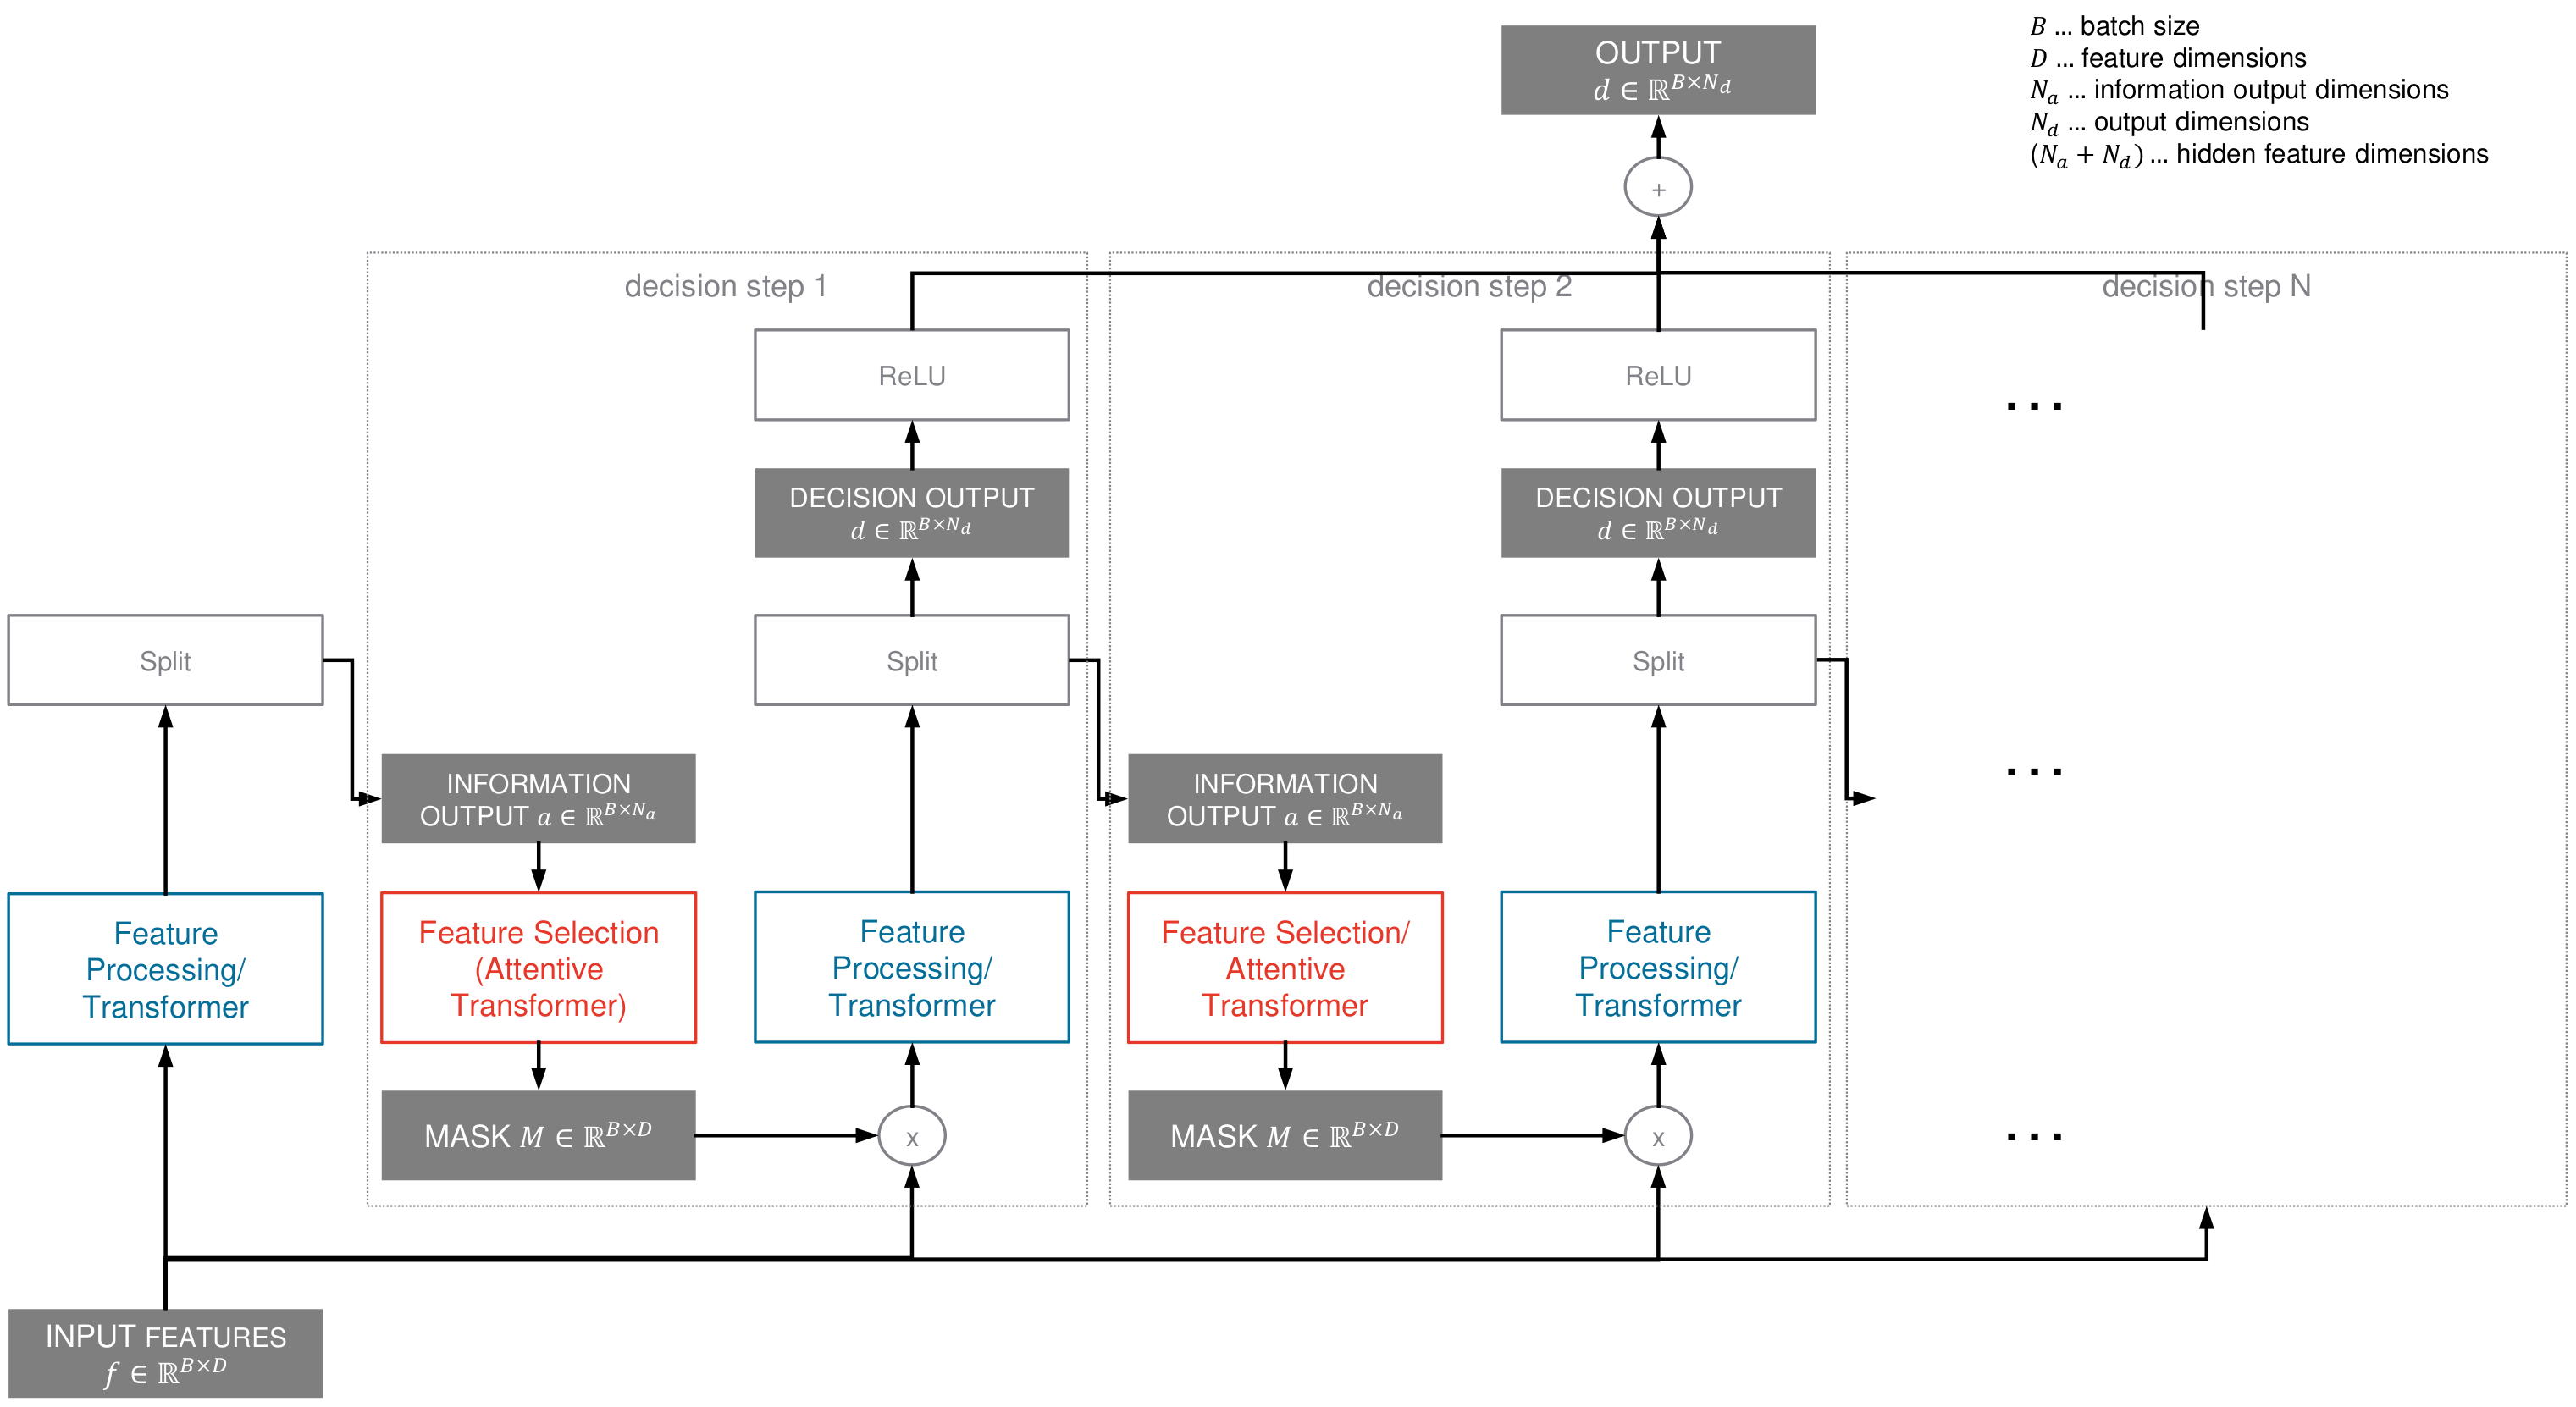
\includegraphics[width=1.0\textwidth]{tabnet}    
    \caption{TabNet architecture overview}
    \label{fig:tabnet}
\end{figure}

In figure \ref{fig:tabnet} the overall TabNet architecture is shown. Inputs to the architecture are in the form $\mathbf{x} \in \mathbb{R}^{B \times D}$, where $B$ refers to the sample size and $D$ determines the number of features or feature dimensions.  Categorical feature dimension are represented as learnable embeddings with dimension size 1. Raw inputs are not globally normalized but batch norm (BN) \cite{ioffe_batch_2015} is applied. Using the batch normalized inputs TabNet uses up to $N_{steps}$ individual blocks called decision steps. Each step $i$ consists of the following components:

\begin{itemize}
    \item \textbf{Attentive Transformer} for feature selection which uses some information or output from the previous decision step $\mathbf{a}^{[i-1]} \in \mathbf{R}^{B\times N_a}$ and a prior scale $\mathbf{P}^{[i-1]} \in \mathbf{R}^{B\times D}$ to determine the features which are processed within the step $i$. The output is a learnable mask $\mathbf{M}^{[i]} \in \mathbf{R}^{B\times D}$ which is used for feature selection.

    \item \textbf{Feature Transformer} for feature processing, using the feature selection mask $\mathbf{M}^{[i]}$ to determine the most salient features for step $i$. Those are selected  using element-wise multiplication with the batch normalized inputs $\mathbf{x}$ in the form $\mathbf{x}_i=\mathbf{M}^{[i]} \odot \mathbf{x}$. 

    \item \textbf{Split} block which separates the feature processing output into two parts the decision output $\mathbf{d}^{[i]} \in \mathbf{R}^{B\times N_d}$ and the information output $\mathbf{a}^{[i]} \in \mathbf{R}^{B\times N_a}$. The dimensions $N_d$ and $N_a$ add up to the overall features dimension $D=N_a+N_d$. The information output $\mathbf{a}^{[i]}$ is used as the input the subsequent step $i+1$. The non-linear activation function \acs{relu} $ReLU = max(0, x)$ is applied to each individual decision output $\mathbf{d}^{[i]}$ and furthermore aggregated with all other decision steps output:

    \begin{equation} \label{eq:d_out}
        \mathbf{d_{out}} = \sum_{i=1}^{N_{steps}} ReLU(\mathbf{d^{[i]}})
    \end{equation}    
\end{itemize}

\subsubsection{Feature Transformer} \label{sssec:feature_transformer}

Each feature transformer (FT) consists of multiple layers. Each layer $l$ consists of a fully connected layer (FC) or linear transformation in the form:

\begin{equation}
    FC_{FT}(\mathbf{x}) = \mathbf{W}^{[l]} \mathbf{x}
\end{equation}

The parameters $\mathbf{W}$ are of dimension $\mathbf{W}^{[1]} \in \mathbb{R}^{H*2 \times D}$ for the first layer connecting input with subsequent layers and $\mathbf{W}^{[l]} \in \mathbb{R}^{H*2 \times H}$ for any following layer $1<l<=N_{layers}$. The dimension $H$ refers to the sum of the decision output dimension $N_d$ and information output dimension $N_a$ as $H = N_d+N_a$. The output of the FC transformation is followed by batch norm (BN). 
\newline

To better support large batch size during training a variant called ghost BN (GBN) is used within the feature transformer. Within BN the statistics for mean $\mu$ and variance $\sigma$ are dependent on the sample or batch size $B$. GBN split the complete batch $B_{complete}$ into $J$ chunks in the form $B_{complete}=[B_1, B_2, \cdots, B_J]$. On each of the chunks the batch statistics are calculated and applied separately such as $[\mu_1, \mu_2, \cdots, \mu_J]$ and $[\sigma_1, \sigma_2, \cdots, \sigma_J]$. Experiments showed that this adaption of BN reduces the generalization error when large batch size are used \cite{hoffer_train_2017}. 
\newline

As non-linearity a gated linear unit (\acs{glu}) \cite{dauphin_language_2017} is used. Given the output of the FC transformation $\mathbf{h} \in \mathbb{R}^{H * 2}$ which is spitted into two parts $\mathbf{h}_a \in \mathbb{R}^H$ and $\mathbf{h}_b \in \mathbb{R}^H$, GLU is defined using a sigmoid activation function $\sigma$, refer to section \ref{par:logreg}, as follows:

\begin{equation}
    GLU(\mathbf{h}) = \mathbf{h}_a \odot \sigma(\mathbf{h}_b)
\end{equation}

The output of the non-linearity is again of size $\mathbb{R}^H$, this also explains the dimensions of the FC transformation above being $H*2$. GLU activation allows unimpeded information flow through the network similar to recurrent neural networks (RNN) with gating mechanism like long short-term memory (\acs{lstm}) \cite{hochreiter_long_1997}. 

Combining those blocks one layer can be summarized as:

\begin{equation}
    L(\mathbf{x}) = GLU(BN(FC_{FT}(\mathbf{x})))
\end{equation}

The output of each layer $l$ is connected the output of the previous layer using skip connection in the form:

\begin{equation}
    L^{[l]}(\mathbf{h}) = \Big( L^{[l]}(\mathbf{h}) + L^{[l-1]}(\mathbf{h}) \Big ) \sqrt{0.5}
\end{equation}

The factor $\sqrt{0.5}$ refers to a normalizing strategy for residual blocks which halves the variance of the sum of both terms \cite{gehring_convolutional_2017}. 

To improve parameter efficiency of TabNet with multiple decision steps layers or more precise the parameters $\mathbf{W}$ of the FC block can be shared over all steps. The following figure \ref{fig:feature_transformer} shows a feature transformer with two shared and two decision step individual layers.

\begin{figure}[H]
    \centering
    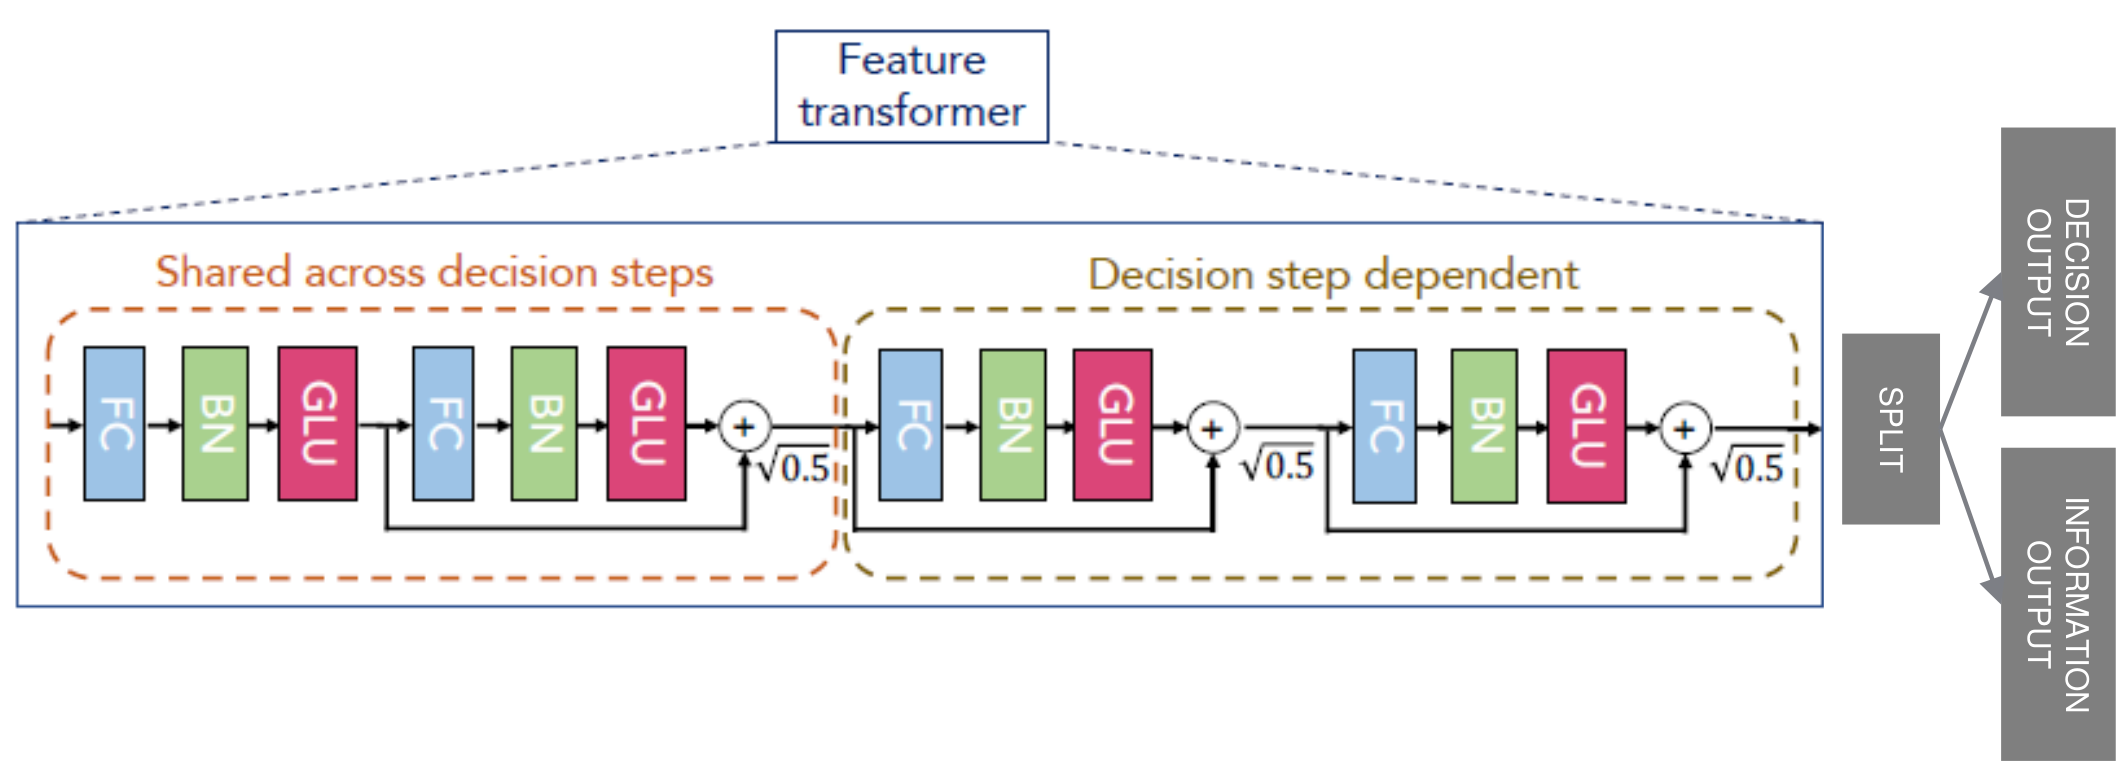
\includegraphics[width=1.0\textwidth]{feature_transformer}    
    \caption{Feature Transformer \cite{arik_tabnet_2020}}
    \label{fig:feature_transformer}
\end{figure}

The final output of feature transformer $\mathbf{h} \in \mathbb{R}^{H}$ is split into two parts, the decision step output $\mathbf{d} \in \mathbb{R}^{N_d}$ and the information which is used in subsequent steps $\mathbf{a} \in \mathbb{R}^{N_a}$. The dimensions add up to the hidden dimension in the form of $H=N_d + N_a$.

\subsubsection{Attentive Transformer} \label{sssec:attentive_transformer}

The output of the previous decision step $\mathbf{a}^{[l-1]}$ is linear transformed followed by ghost BN, refer to section \ref{sssec:feature_transformer}, in the form:

\begin{equation}
    FC(\mathbf{a}^{[l-1]})=BN(\mathbf{V^{[l]}\mathbf{a}^{[l-1]}})
\end{equation}

$\mathbf{V^{[l]}}$ describes the learnable parameters within the attentive transformer which subsequent determine which features are selected. The output of $FC(\mathbf{a}^{[l-1]})$ is multiplied with a prior scale term $\mathbf{P}^{[l-1]}$ which indicates what features have been used in previous decision steps. Finally the non-linear transformation $sparsemax$ is applied as follows which results in the feature selection mask $M^{[l]}$:

\begin{equation}
    \mathbf{M}^{[l]}=sparsemax(\mathbf{P}^{[l-1]} \odot FC(\mathbf{a}^{[l-1]}))
\end{equation}

The output of $sparsemax$ is a probability distribution with the property $\sum_{j=1}^{D} M^{[l]}_{b,j}=1$, refer to section \ref{sssec:sparsemax}. Additionally, $sparsemax$ can output sparse probability meaning some entries $j\in D | M^{[l]}_{b,j}=0$.

Given the relaxation parameter $\gamma$ $\mathbf{P}^{[l]}$ is given as:

\begin{equation} \label{eq:gamma}
    \mathbf{P}^{[l]}=\prod_{j=1}^{l}(\gamma - \mathbf{M}^{[j]})
\end{equation}

The relaxation parameter $\gamma$ indicates if a feature is more likely used in more than one decision step. Starting from $\gamma = 1$ more flexibility in reusing features over multiple decision steps is provided as its value increases.

To further control sparsity TabNet propose to add a sparsity regularization term in form of entropy to the overall loss, with $\epsilon$ for numerical stability:

\begin{equation} \label{eq:sparsity_regularization}
    L_{sparse}=\sum_{l=1}^{N_{steps}} \sum_{b=1}^B \sum_{j=1}^D \frac{-M^{[l]}_{b,j} log(M^{[l]}_{b,j} + \epsilon )}{N_{steps} \cdot B}
\end{equation}

The effect of sparsity regularization can be controlled with $\lambda_{sparse}$ and is used in the overall loss term:

\begin{equation} \label{eq:lambda_sparse}
    L=L+\lambda_{sparse}L_{sparse}
\end{equation}

High values for $\lambda_{sparse} \uparrow$ encourage more sparsity of $\mathbf{M} \uparrow$ $\downarrow$ while values approaching 0 for $lambda_{sparse} \downarrow$ result in less sparsity.

%TODO rewrite sparsity regularization

%%%%%%%%%%%%%%%%%%%%%%

\subsubsection{Sparsemax} \label{sssec:sparsemax}

Sparsemax activation function was introduced by Martins A. and Astudillo R. in 2016 \cite{martins_softmax_2016}. Similar to $softmax$ the output follows a probability distribution. Given the input vector $\mathbf{z} \in \mathbb{R}^K$ first recap $softmax$ which is defined for $i=1,\ldots,K$ as:

\begin{equation}
    softmax(\mathbf{z})_{i}=\frac{e^{z_i}}{\sum_{j=1}^{K}e^{z_j}}
\end{equation}

As already mentioned the output $\mathbf{o} \in \mathbb{R}^K$ of $softmax(\mathbf{z})$ follows a probability distribution having the property $\sum_{i=1}^{K}o_i = 1$. As $softmax$ is fully differentiable the gradient of $softmax(\mathbf{z})_i$ w.r.t. one particular entry $z_j$ is given as:

\begin{equation}
    \frac{\partial softmax(\mathbf{z})_i}{\partial z_j} = softmax(\mathbf{z})_i(\delta_{ij}-softmax(\mathbf{z})_j)
\end{equation}

$\delta_{ij}$ refers to the Kronecker delta which is defined as 1 if two variables $i$ and $j$ are equal and 0 otherwise:

\begin{equation}
    \delta_{ij}=
    \begin{cases}
        1,& \text{if } i=j \\
        0,& \text{otherwise } \\
    \end{cases}
\end{equation}

The full Jacobian $J_{softmax(\mathbf{z})} \in \mathbb{R}^{K \times K}$ using the defined output $\mathbf{o}=softmax(\mathbf{z})$ is given as follows:

\begin{equation}
    J_{softmax(\mathbf{z})}=diag(\mathbf{o})-\mathbf{o}\mathbf{o}^T
\end{equation}

In contrast to $softmax$ which has full support meaning $softmax(\mathbf{z})_i \ne 0, \text{ for }$ $sparsemax$ can output a sparse probability distribution and is defined as follows:

\begin{equation} \label{eq:sparsemax}
    sparsemax(\mathbf{z})=\underset{\mathbf{p} \in \Delta^{K-1}}{argmin} \lVert \mathbf{p} - \mathbf{z} \rVert ^ 2
\end{equation}

This describes the Euclidean projection of the input $\mathbf{z}$ onto the probability simplex. A probability simplex refers to the geometric representation of a probability distribution in the form of a polytope, meaning an object having flat sides. The simplex $\Delta ^ {K-1}$ refers to $K-1$ dimensional object having $K$ corners or vertices, e.g. $\Delta ^ {2}$ refers to a line, $\Delta ^ {3}$ refers to triangle and so on. For a probability simplex each corner represents the probability of a specific event or case $k\in K$. 
\newline

For equation \ref{eq:sparsemax} closed form solution exists. One simple solution is described in algorithm \ref{alg:sparsemax}.

\begin{algorithm}[H]
    \caption{Sparsemax closed form solution \cite{martins_softmax_2016}} \label{alg:sparsemax}
    \begin{algorithmic}[1]
    
        \Require Given input vector $\mathbf{z} \in \mathbb{R}^K$
        \Require Define vector $[K] = [1,2,\cdots,K]$

        \State Sort $\mathbf{z}$ in in descending order: $\mathbf{z}_{s}=[z_{(1)} \ge \cdots \ge z_{(K)}]$
        
        \State Find max index $k \in [K]$ for which $1+k\cdot z_{s(k)}$ is still greater than the cumulative sum of $\mathbf{z}_{s}$ until index $k$, this can be expressed as function $k(\mathbf{z}_{s})$:

        $k(\mathbf{z}_s)=max \Big\{ k \in [K] | 1+k\cdot z_{s(k)} > \sum_{j \le k} z_{s (j)} \Big\}$

        \State Compute the threshold $\tau(\mathbf{z})$ as the cumulative sum of $\mathbf{z}_{s}$ until the max support index $k(\mathbf{z}_{s})$ minus $1$ divided by the max index $k(\mathbf{z}_{s})$:
        
        $\tau(\mathbf{z})=\frac{(\sum_{j \le k(\mathbf{z}_{s})}z_{j}) - 1}{k(\mathbf{z}_{s})}$
        
        \State \Return $max(0, z_i - \tau(\mathbf{z}))$   

    \end{algorithmic}
\end{algorithm}

Furthermore the support $S$ of $sparsemax$ is defined as all indices, for which the return value is above 0: 

\begin{equation}
    S(\mathbf{z}) = [i \in [K] | sparsemax(\mathbf{z})_i > 0]
\end{equation}

Sparsemax is differentiable everywhere except at splitting points, similar to the activation functions ReLU which is not differentiable when evaluated at 0. Therefore the gradient of $sparsemax(\mathbf{z})_i$ w.r.t. $z_j$ following \cite{martins_softmax_2016} is defined as:

\begin{equation}
    \frac{\partial sparsemax(\mathbf{z})_i}{\partial z_j} = 
    \begin{cases}
        \delta_{ij} - \frac{\partial \tau(\mathbf{z})}{\partial z_j},& \text{if } z_i > \tau(\mathbf{z}) \\
        0,& \text{otherwise } \\
    \end{cases}
\end{equation}

\begin{equation}
    \frac{\partial \tau(\mathbf{z})}{\partial z_j} = 
    \begin{cases}
        \frac{1}{|S(\mathbf{z})|},& \text{if } j \in S(\mathbf{z}) \\
        0,& \text{otherwise } \\
    \end{cases}
\end{equation}

Given $z_j > \tau(\mathbf{z})$ if $j \in S(\mathbf{z})$:

\begin{equation}
    \frac{\partial sparsemax(\mathbf{z})_i}{\partial z_j} = 
    \begin{cases}
        \delta_{ij} - \frac{1}{|S(\mathbf{z})|},& \text{if } i,j \in S(\mathbf{z}) \\
        0,& \text{otherwise } \\
    \end{cases}
\end{equation}

The Jacobian $J_{sparsemax(\mathbf{z})} \in \mathbb{R}^{K \times K}$ using the the support function $S(\mathbf{z})$ in form of $\mathbf{s}=[1 \text{ if } i \in S(\mathbf{z}) \text{ otherwise } 0 \text{ for all } i \in K]$ can be calculated as:

\begin{equation}
    J_{sparsemax(\mathbf{z})}=diag(\mathbf{s})-\frac{\mathbf{s}\mathbf{s}^T}{|S(\mathbf{z})|}
\end{equation}

In the two-dimensional case softmax and sparsemax collapse to sigmoid and hard-sigmoid respectively. This can be seen in figure \ref{fig:softmax_sparsemax} presenting $softmax([t,0])_1$ and $sparsemax([t,0])_1$ in blue, plus their derivations $\frac{\partial softmax([t,0])_1}{\partial t}$ and $\frac{\partial sparsemax([t,0])_1}{\partial t}$ in orange.

\begin{figure}[H]
    \centering
    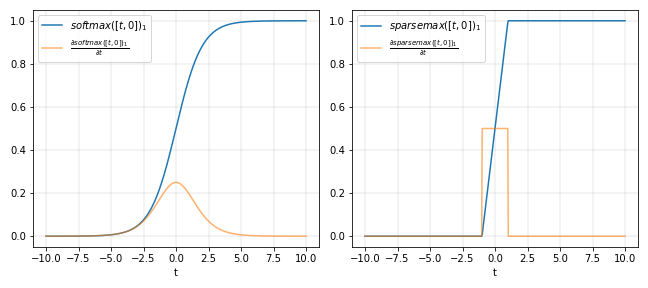
\includegraphics[width=0.9\textwidth]{softmax_sparsemax}    
    \caption{Softmax and sparsemax}
    \label{fig:softmax_sparsemax}
\end{figure}

Further work by Peters B. et al. \cite{peters_sparse_2019} pointed out that softmax and sparsemax both can be expressed as a projection of an input vector $\mathbf{z} \in \mathbb{R}^K$ on a probability simplex which only differ in the choice of entropy regularization.

\begin{equation}
    \begin{aligned}
        softmax(\mathbf{z}) &= \underset{\mathbf{p} \in \Delta^d}{argmax} (\mathbf{p}^T\mathbf{z}+H^S(\mathbf{p})) \\
        sparsemax(\mathbf{z}) &= \underset{\mathbf{p} \in \Delta^d}{argmax} (\mathbf{p}^T\mathbf{z}+H^G(\mathbf{p}))
    \end{aligned}
\end{equation}

Softmax is using Shannon entropy $H^S(\mathbf{p})=-\sum_{j}p_j log(p_j)$ while sparsemax uses Gini entropy $H^G(\mathbf{p})=\frac{1}{2}\sum_j p_j (1-p_j)$. Using a generalized form of entropy called Tsallis $\alpha$ entropy which is defined as:

\begin{equation}
    H^T_\alpha(\mathbf{p}) =
    \begin{cases}
        \frac{1}{\alpha (\alpha - 1)} \sum_j (p_j-p_j^{\alpha}) ,& \alpha \ne 1 \\
        H^S(\mathbf{p}),& \alpha=1 \\
    \end{cases}
\end{equation}

Using Tsallis entropy a generalized or interpolated version of softmax and sparsemax called $\alpha-entmax$ can be defined:

\begin{equation}
    \alpha-entmax(\mathbf{z}) = \underset{\mathbf{p} \in \Delta^d}{argmax} (\mathbf{p}^T\mathbf{z}+H^T_{\alpha}(\mathbf{p})) \\            
\end{equation}

Depending on $\alpha$ outputs are more $\alpha \uparrow$ or less sparse $\alpha \downarrow$. $\alpha-entmax$ is differentiable also w.r.t. $\alpha$ itself. Even though $\alpha-entmax$ was not applied within TabNet it is mentioned here as a generalization of sparsemax. Furthermore in figure \ref{fig:entmax} the two dimensional case $[t,0]$ with different values for $\alpha$ with the corresponding gradients w.r.t. $t$ is shown. 

\begin{figure}[H]
    \centering
    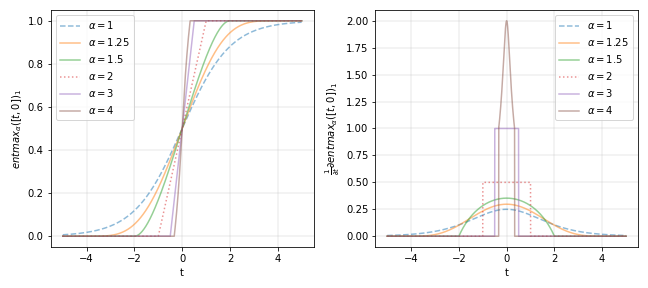
\includegraphics[width=0.9\textwidth]{entmax}    
    \caption{$\alpha-entmax$ evaluation and gradients}
    \label{fig:entmax}
\end{figure}

\subsubsection{Interpretability} \label{sssec:interpretability}

Before any input is processed within a decision step $l$, the input is multiplied with the sparse probability feature selection mask $\mathbf{M}^{[l]}$ as described in section \ref{sssec:attentive_transformer}. Therefore TabNet by design explains which features are used to determine the output or prediction and which are not. As the overall TabNet output is a linear combination of the individual decision steps outputs as shown in \ref{eq:d_out} the overall aggregated feature mask must also take into account the individual decision step contribution. Therefore for one concrete sample $b$ a coefficient term $\eta_b^{[l]}$ is calculated as follows:

\begin{equation}
    \eta_b^{[l]} = \sum_{i=1}^{N_d} ReLU(d_{b, i}^{[l]})
\end{equation}

This coefficient or scale term $\eta_b^{[l]}$ determines the importance or contribution of one particular decision step $l$ and is used to scale the impact of the corresponding feature selection mask $\mathbf{M}^{[l]}$ accordingly. Using this scale term the overall feature importance or contribution mask $M_{agg, b}$ is given as follows:

\begin{equation} \label{eq:aggregated_mask}
    \mathbf{M}_{agg, b} = \sum_{i=1}^{N_d} \eta_b^{[l]} \mathbf{M}^{[l]}
\end{equation}

Beside the overall feature selection and attribution using $\mathbf{M_{agg}}$, TabNet allows insight which features together have been used in an individual step by just looking at individual feature selection masks $\mathbf{M}^{[l]}$. This design allows for a potential better interpretability of interactions of features within the TabNet architecture. This is additionally presented in the following figure \ref{fig:tabnet_interpret}. 

\begin{figure}[H]
    \centering
    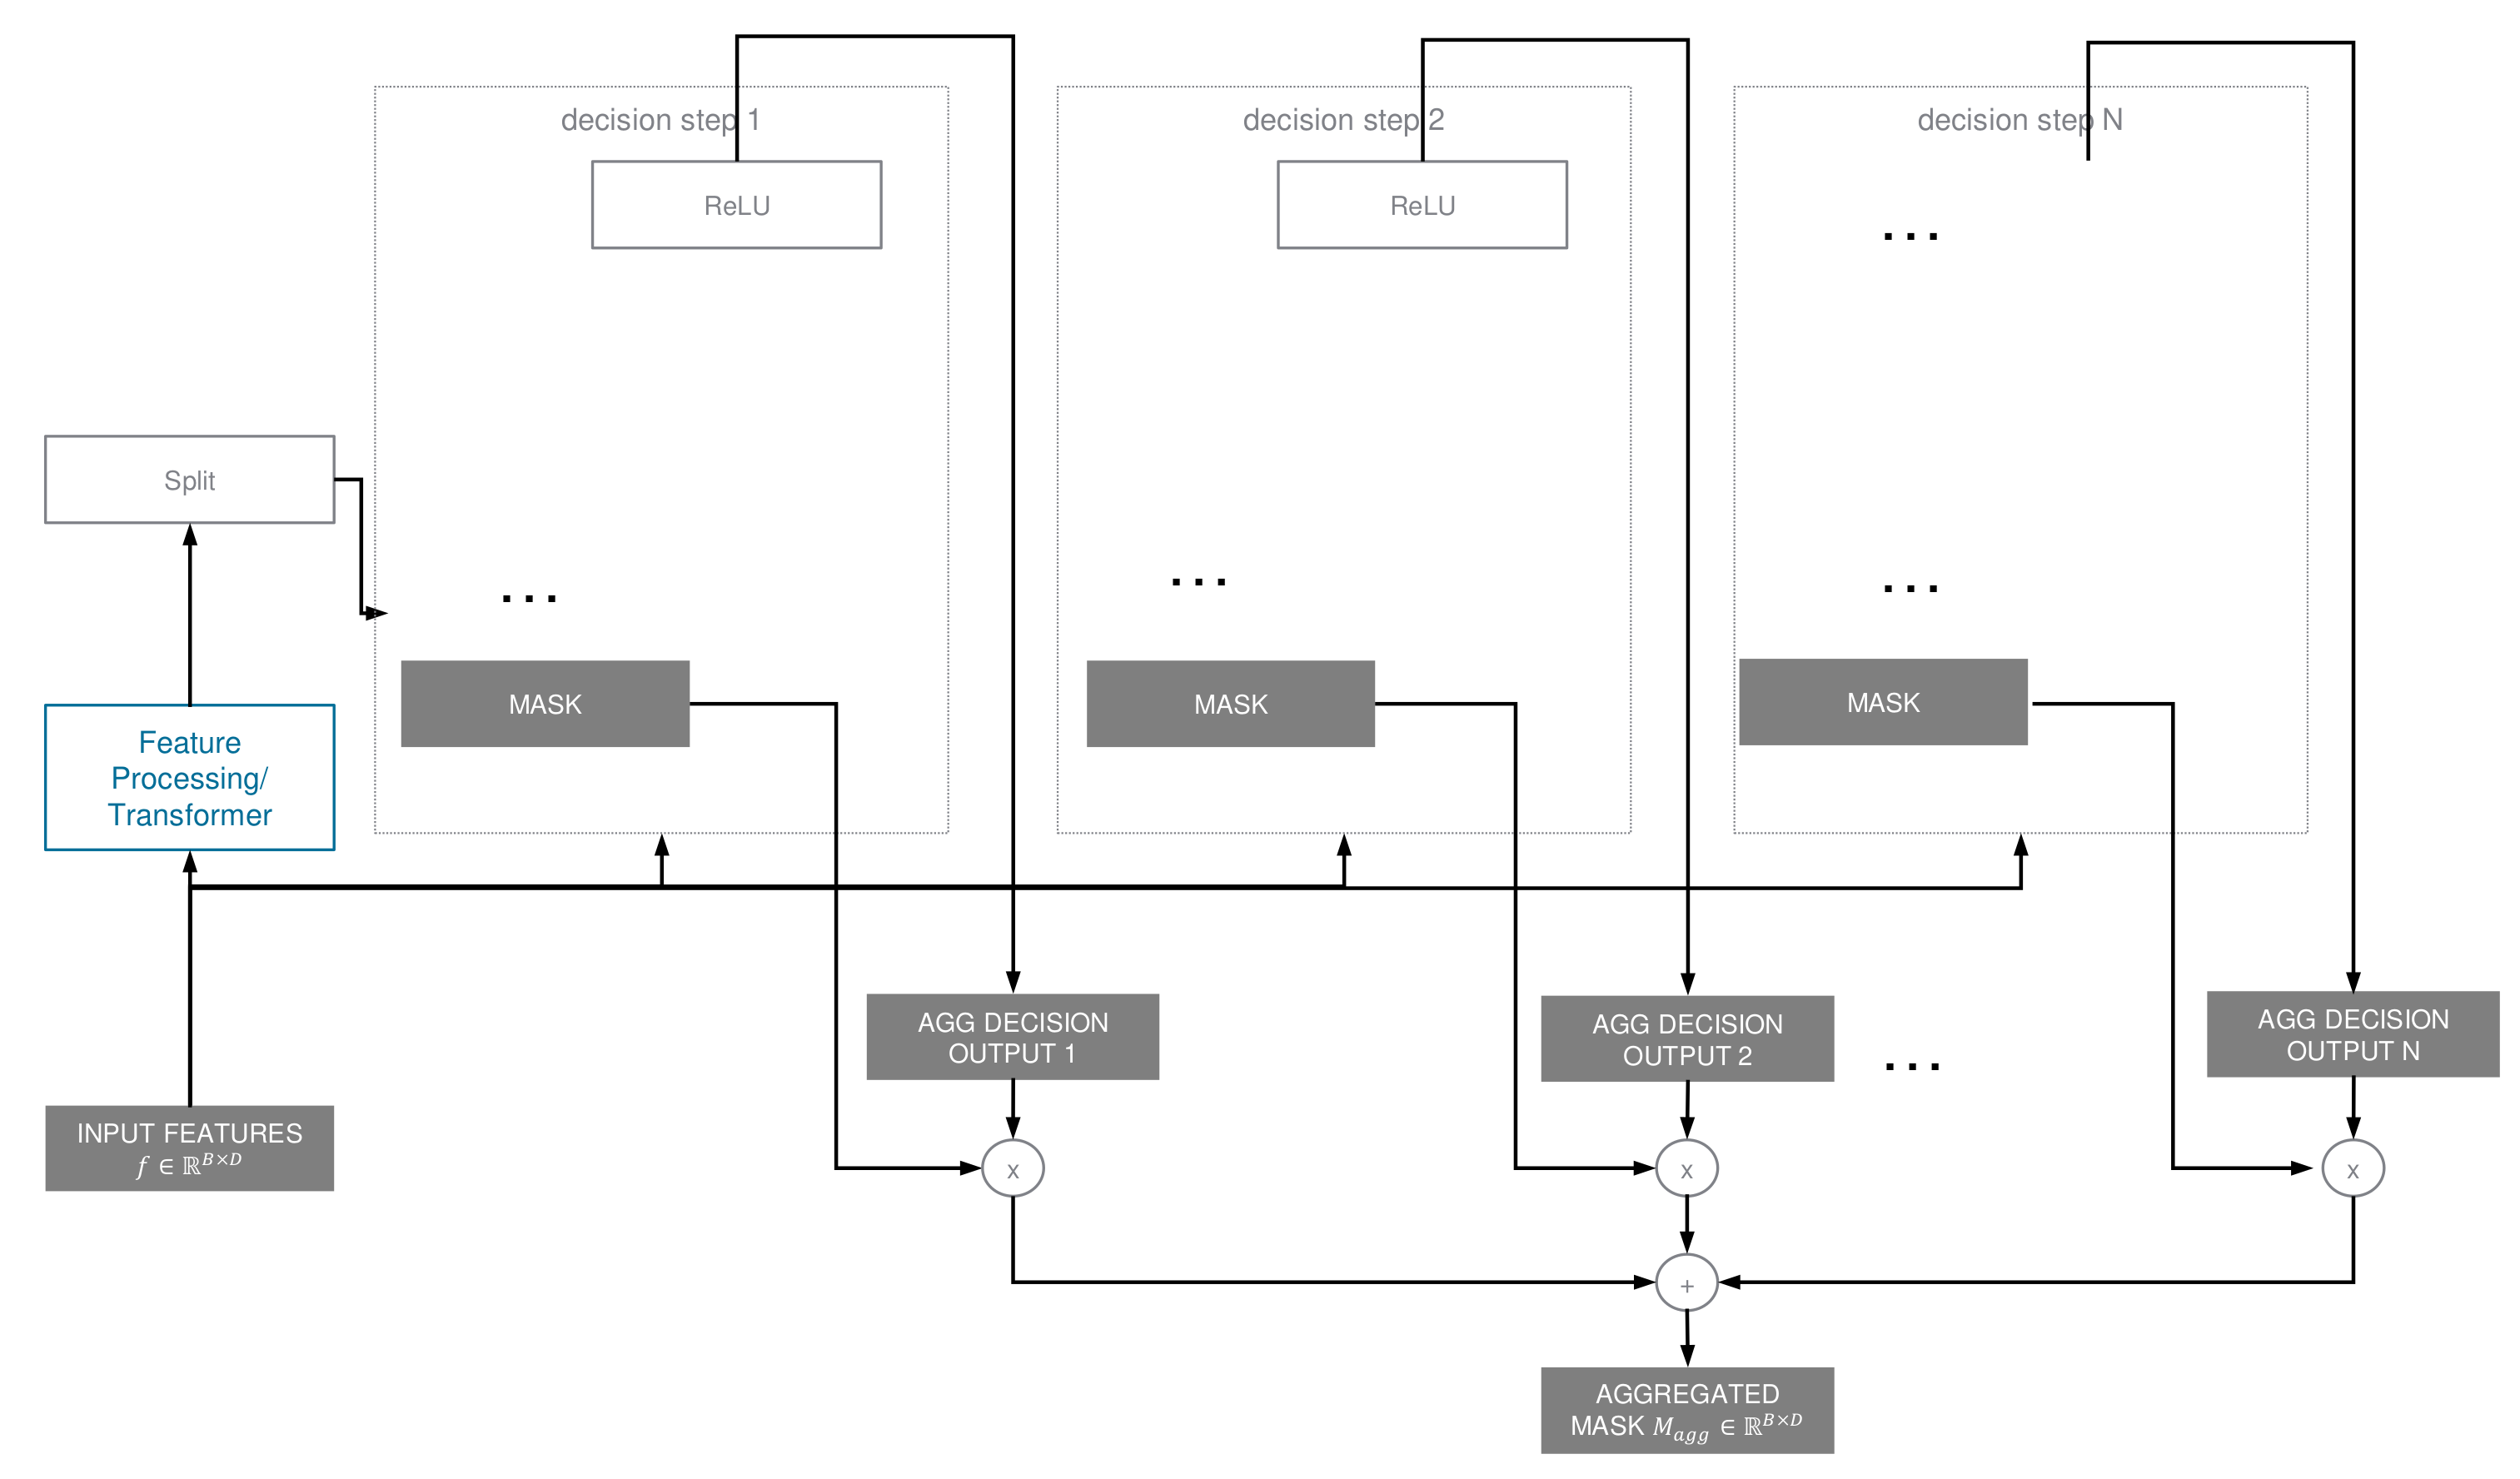
\includegraphics[width=0.9\textwidth]{tabnet_interpret}    
    \caption{TabNet interpretability overview}
    \label{fig:tabnet_interpret}
\end{figure}

Even though TabNet by design returns the selected features and their contribution to achieve a defined objective, it does not give an insight into the feature selection process itself. The question why a particular feature was not selected, e.g. because of the presence or absence of another feature can not be answered by TabNet directly. 

\newpage

\subsection{Machine Learning Interpretability Methods} \label{ssec:interpret_methods}

Beside the concrete result of a machine learning method, for humans to interpret the outcome, or get a more in depth explanation why a particular result was achieved is crucial. Especially for tasks in high stake domains like healthcare, medical research, security applications and many others. Recent developments in machine learning and in deep learning lead to complex models with billions of parameters which in many cases achieved state-of-the-art results but are also difficult or not at all to interpret \cite{linardatos_explainable_2021}.
To tackle this and other problems the research stream of explainable artificial intelligence (\acs{xai}) become more important in recent years. Even though there exists attempts \cite{palacio_xai_2021}, \cite{barredo_arrieta_explainable_2020} to define XAI and terms such as  "explainability" and "interpretability" a common agreed upon definition does not exists and those terms often are used interchangeably \cite{marcinkevics_interpretability_2020}. Nonetheless agreed upon goals and concepts of XAI can be found. Following the DARPA (US Defense Advanced Research Projects Agency) XAI should "produce more explainable models while maintaining high level of learning performance and enable human users to understand, appropriately trust, and effectively manage the emerging generation of artificially intelligent partners" \cite{darpa_xai}. 
When looking at concepts and problems which are subject of research within XAI the following can be found \cite{lipton_mythos_2017}.

\begin{itemize}
    \item \textbf{Trust} refers to an idea that results of a model must be trustworthy. This is usually measured using the raw performance or accuracy numbers of a model. But trust is also important in context of bias or imbalance within training data and how this problem is being addressed. Furthermore, beside the raw performance, it is also important to know for which examples or in which situation a model is more prone to errors. 

    \item \textbf{Causality} describes the concept to infer causal relationships between input data from a model which function as the basis for further research hypothesis. 

    \item \textbf{Informativeness} of a model is given if a human is able to extract additional information beside the raw output or prediction from a model.

    \item \textbf{Justification} is based on the idea of fair and ethical decision making. In the context of regulation for example the European Union stresses that individual effected by algorithm decisions have the right for explanation. The question why a prediction or output was generated by a model must be explained, based on a falsifiable proposition which provides a way to contest those proposition. 

    \item \textbf{Transparency} of how a model outcome or prediction was determined. It refers to the problem that many machine learning models don't offer interpretability or explainability by design but function as a black-box which uses input data to determine an output or prediction. Without further tools or method transparency of the internal functionality is not given.

\end{itemize}

Enabling XAI and especially supporting transparency requires concrete interpretability methods and concepts.  Therefore to further categorize interpretability methods the taxonomy shown in figure \ref{fig:interpret_methods} is presented.

\begin{figure}[H]
    \centering
    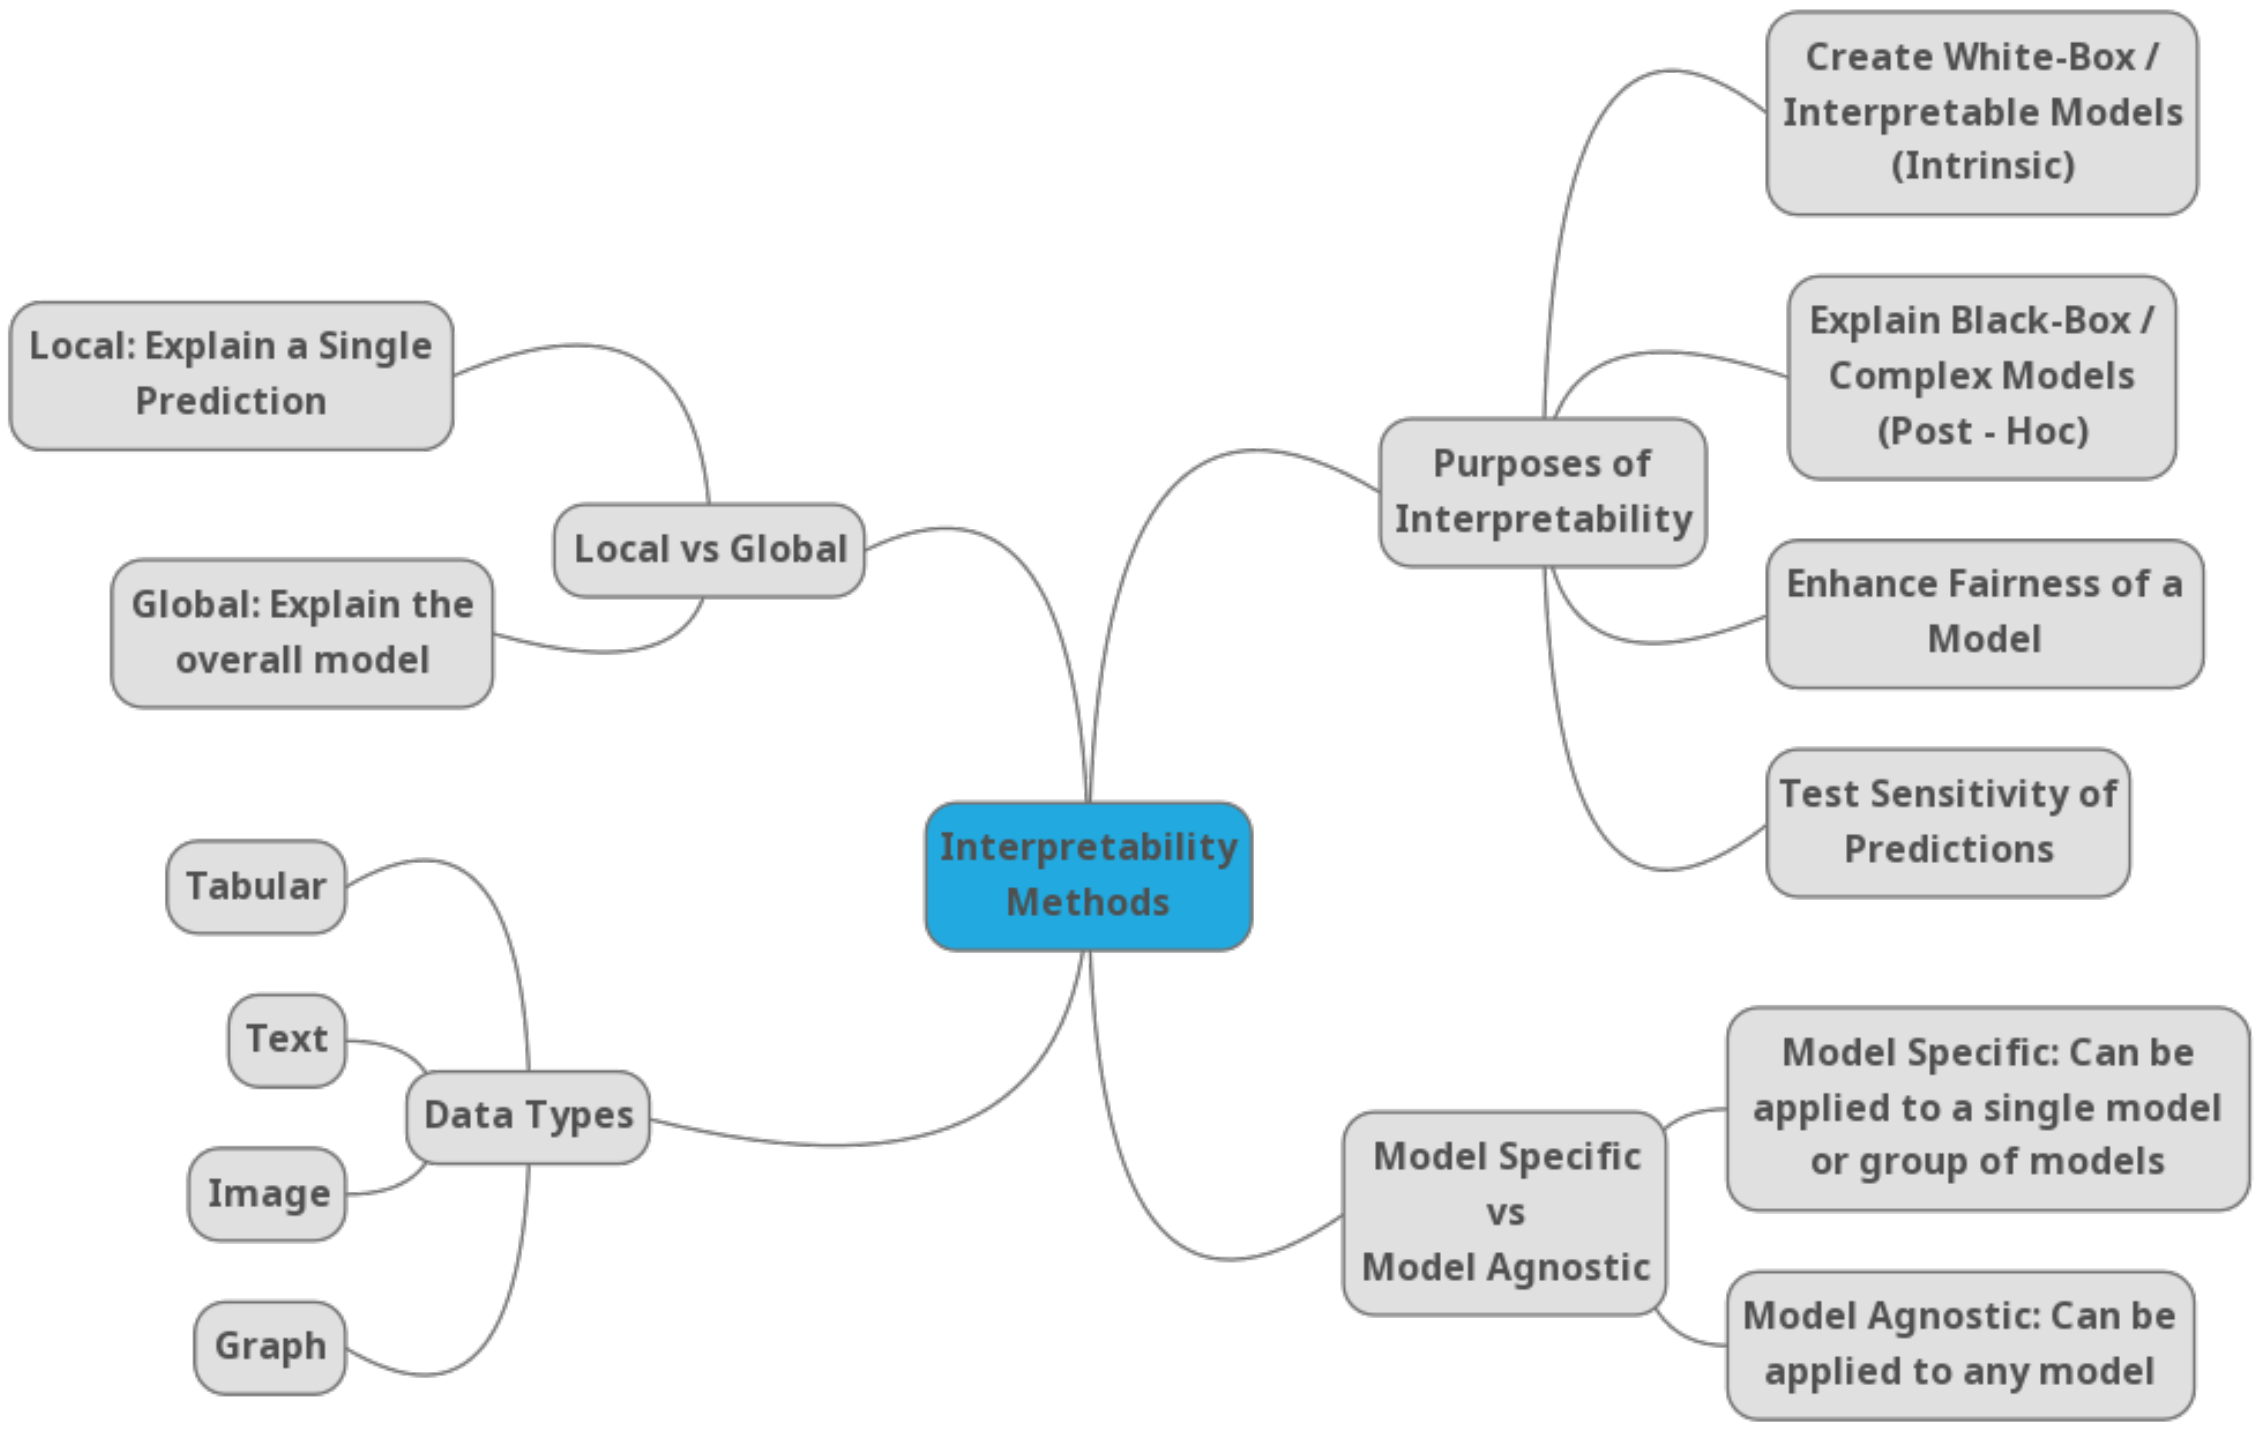
\includegraphics[width=0.9\textwidth]{interpret_methods}    
    \caption{Taxonomy of interpretability methods \cite{linardatos_explainable_2021}}
    \label{fig:interpret_methods}
\end{figure}

Focusing on the categories "Local vs Global", "Model Specific vs Model Agnostic" and "Post-hoc Methods" the following sub chapters outline some recent implementations of interpretability methods focusing on deep learning architectures. A common task for interpretability methods is given a model $f \mid \mathbf{x} \rightarrow \mathbf{y} $ mapping from $\mathbf{x} \in \mathbb{R}^D$ to $\mathbf{y} \in \mathbb{R}^K$ find the feature attribution $\mathbf{a} \in \mathbb{R}^K$ using interpretability method $A \mid \mathbf{x} \rightarrow \mathbf{a}$ such that for each feature $[x_1, \ldots, x_D]$ there exists a attribution value $[a_1, \ldots, a_D]$ describing the contribution of each feature to the model output or prediction $\mathbf{y}$. This task is also referred to as feature attribution.

\subsubsection{Integrated Gradients}

Integrated gradients (\acs{ig}) offers local feature attribution and is specific to models which are trained using gradient descent. Original introduced in 2017 \cite{sundararajan_axiomatic_2017} it became one of the most prominent feature attribution method. IG requires the definition of a baseline $x'$ which is used to generate interpolations between $\mathbf{x}'$ and the actual input data $\mathbf{x}$. Using the interpolations the gradients of a model $F$ w.r.t. $\mathbf{x}$ are calculated and aggregated. The following equation describes the calculation of IG for one particular feature dimension $d$ within $\mathbf{x} \in \mathbb{R}^D$:

\begin{equation}
    IG_d(\mathbf{x}) = (x_d - x'_d) \int_{\alpha=0}^1 \frac {\partial F(\mathbf{x}'+\alpha (\mathbf{x}-\mathbf{x}'))}{\partial x_d} d\alpha
\end{equation}

Due to difficulties calculation the integral for numerical reasons often an approximation using Riemann sum with $m$ steps is used:

\begin{equation}
    IG_d^{approx}(\mathbf{x}) = (x_d - x'_d) \sum_{k=1}^m \frac {\partial F(\mathbf{x}'+\frac{k}{m} (\mathbf{x}-\mathbf{x}'))}{\partial x_d} \frac{1}{m}
\end{equation}

IG results in local or instance wise feature attribution values. Global feature attribution for a model can not be determined. Additionally relations or interactions between features can not be explained. 

\subsubsection{Saliency}

The concept of saliency for feature attribution was first introduces in 2014 \cite{simonyan_deep_2014} in the context of computer vision to provide saliency maps of pixels contributing the most to a given prediction. Saliency provides local feature attribution values for gradient based methods. The idea is to use the gradient $\mathbf{w}$ of the model $f_c$ for a concrete output or class $c$ w.r.t. its input $\mathbf{x} \in \mathbb{R}^D$ to approximate the function output $f_c$ by using a first-order Taylor expansion:

\begin{equation}
    f_c(\mathbf{x}) \approx \mathbf{w}^T \mathbf{x} + b
\end{equation}

The gradient $\mathbf{w} \in \mathbb{R}^D$ is given as:

\begin{equation}
    \mathbf{w}=\frac{\partial f_c}{\partial \mathbf{x}}
\end{equation}

The feature attribution values are given by either using the absolute gradient values $|\mathbf{w}|$, or the gradients $\mathbf{w}$ directly (relative). Saliency is an easy to compute feature attribution method but similar to IG does not describe relationships or interactions between features. Additionally, it suffers from the problem of saturated gradients which is relevant for models using ReLU activation \cite{shrikumar_learning_2017}.

\subsubsection{Shapley Values}

The original concept was introduced in 1951 by Lloyd Shapley \cite{shapley1951notes} and tried to solve the problem of a fair and equal payment schema between participants who together produces a certain value or outcome. Similarly within a machine learning model the input data consists of multiple participants or feature dimensions which together produce an outcome or prediction. Therefore Shapley values can be used to identify the individual feature attribution or contribution to the overall model outcome. It produces local or instance wise feature attribution but in contrast to gradient based method is model agnostic. 
Given input data $\mathbf{x} \in \mathbb{R}^D$ having $D$ dimensions which contribute to the outcome of a model $f$ the Shapley value for the $i$ feature or dimension can be written down as:

\begin{equation}    
    \psi_{i}(f) = \frac{1}{D} \sum_{\mathbf{s}\subseteq \mathbf{x} \setminus \{x_i\}} \binom{D - 1}{|\mathbf{s}|}^{-1} \Big( f(\mathbf{s} \cup x_i ) - f(\mathbf{s}) \Big)
\end{equation}

The term $\mathbf{s} \subseteq \mathbf{x} \setminus \{x_i\}$ refers to a subset of features without the feature $x_i$ for which the Shapley value is calculated. As the input to the model $f$ is of dimension $D$ the vector representing the subset $\mathbf{s} \in \mathbb{R}^D$ is also of the same size. In practice a baseline value (e.g. zero) is used replacing entries not present in the corresponding subset $\mathbf{s}$. For example given $\mathbf{x}=[x_1, x_2, x_3]$ there are 4 possible subsets excluding $x_1$ using zero as a baseline value, $\mathbf{s}_0 = [0, 0, 0]$,  $\mathbf{s}_1 = [0, x_2, 0]$, $\mathbf{s}_2 = [0, 0, x_3]$ and $\mathbf{s}_3 = [0, x_2, x_3]$. 
\newline

The marginal value or contribution when adding $x_i$ is given by $f(\mathbf{s} \cup  x_i ) - f(\mathbf{s})$. It calculates the output for a given subset $\mathbf{s}$ including feature $x_i$ minus the output using just the subset $\mathbf{s}$. The term $\binom{D - 1}{|\mathbf{s}|}^{-1}$ uses the number of combinations for the amount of features in $|\mathbf{s}|$ to scale the marginal contribution of $x_i$. For the mentioned example this results in the individual marginal values of $1 \cdot f([x_1, 0, 0]) - f([0, 0, 0])$, $\frac{1}{2} \cdot f([x_1, x_2, 0]) - f([0, x_2, 0])$, $\frac{1}{2} \cdot f([x_1, 0, x_3]) - f([0, 0, x_3])$, $1 \cdot f([x_1, x_2, x_3]) - f([0, x_2, x_3])$. Finally the individual marginal values are aggregated and scaled by $\frac{1}{D}$. 

Given $D$ feature dimension calculating the Shapley values requires $2^D$ subsets which needs to be considered. For many real world applications this is computational not feasible. In practice Shapley values are estimated using various techniques. One simple one is to only consider a sample of available subsets for calculations, this is also referred to as Shapley value sampling \cite{castro_polynomial_2009}.

\subsection{Drug Discovery} \label{ssec:drug_discovery}

Development of new drugs is a complex and costly process having R\&D costs of 2.6 billion USD per newly developed drug. The whole process until approval takes about 13.5 years, with 5.5 years before any clinical trails, also referred to as drug discovery process and 8 years for the remaining preclinical, clinical and approval phases \cite{kim_artificial_2020}.

Development of a new drug for a a selected disease starts with identification and validation of a potential target candidates. Based on the exploratory research results target candidates are tested in large screening tests to identify possible molecules which have desired affinity with the target. Those molecules referred to as HIT molecules are further analyzed to identify a lead compound which modify bind to targets in specific and selective way and modify its normal mechanism of action. The lead compound is further modified to improve its general biological activity as well as absorption, distribution, metabolism and excretion (ADME) behavior. If a promising lead compound could be successfully identified and modified pre-clinical and clinical trials phases starts \cite{duelen_medicinal_2019}. In the following figure \ref{fig:drug_discovery_process} an overview of the process is presented.

\begin{figure}[H]
    \centering
    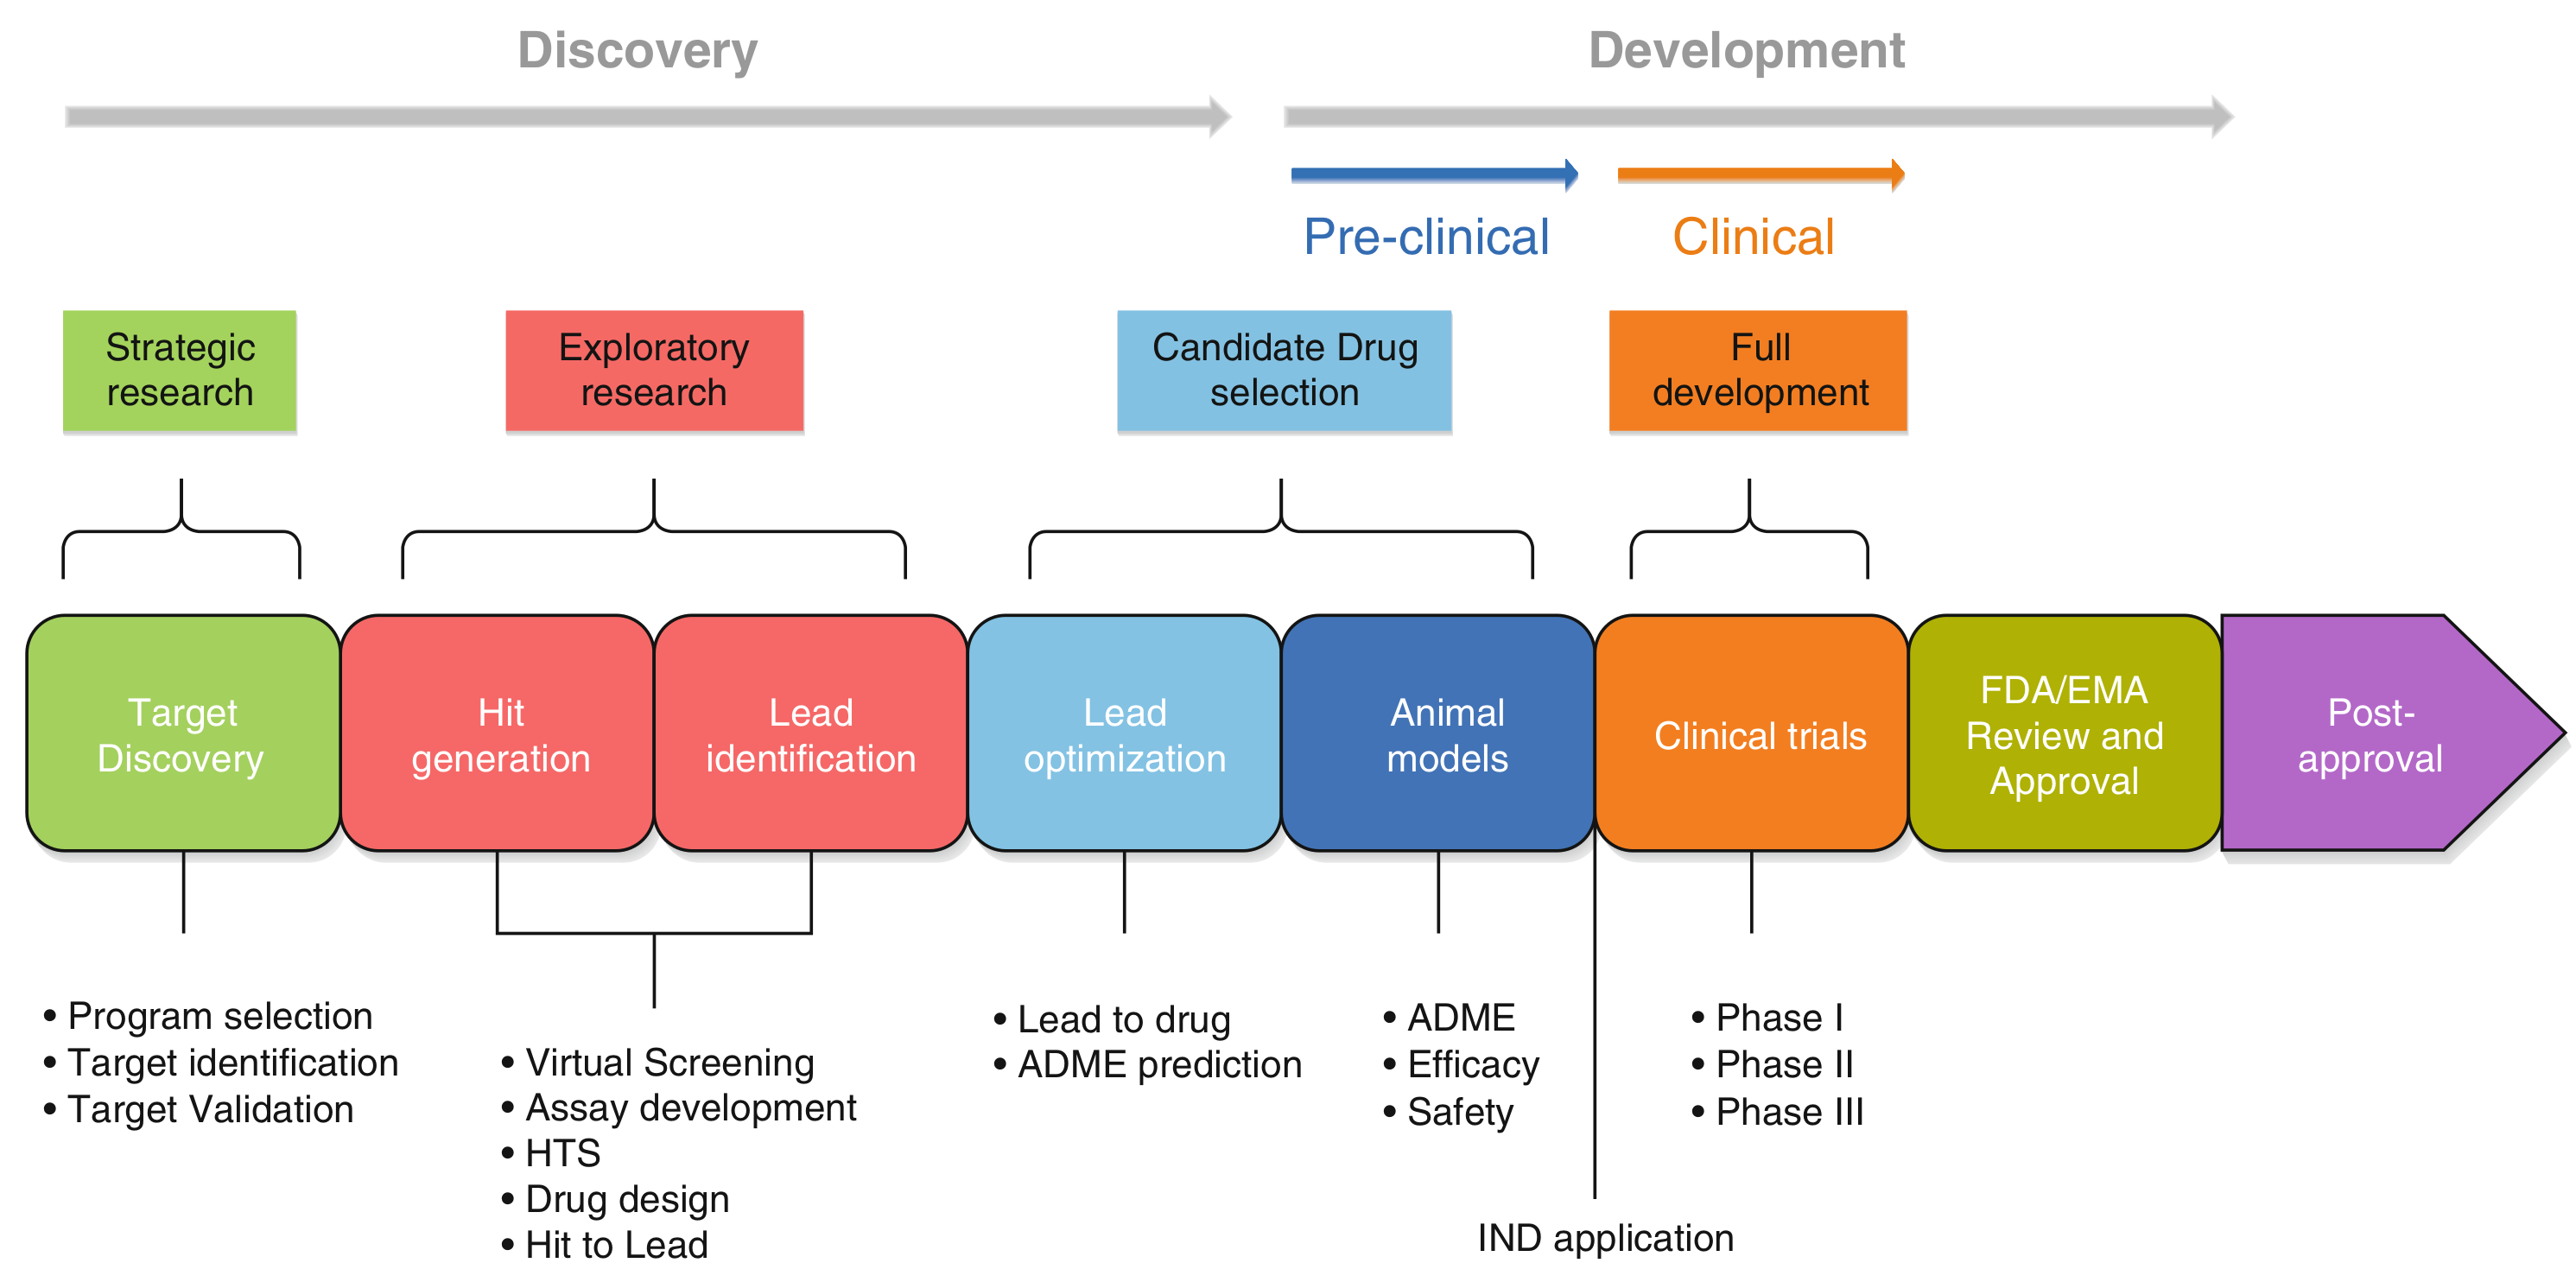
\includegraphics[width=0.9\textwidth]{drug_discovery_process}    
    \caption{Drug development and discovery process overview \cite{duelen_medicinal_2019}}
    \label{fig:drug_discovery_process}
\end{figure}

During the drug discovery process various assays are applied which can be categorized by the type or environment the are carried out:

\begin{enumerate}
    \item \textbf{In-vitro} ("in glass") - refers to an assay performed in wet lab in which in the context of drug discovery a molecule or ligand is tested for a desired biological effect onto a target.
    \item \textbf{In-vivo} ("in the living") - describes an assay performed on living organisms (e.g. plants, animals).
    \item \textbf{In-silico} - describes assays performed by computational simulations.
\end{enumerate}

Especially in-silico assay helps to reduce the quantity of molecules which are candidates for further test in-vitro assays and therefore reduce the costs of drug discovery and development. This leads to an every increasing number of companies developing and applying ML and AI methods within the drug discovery process\cite{duelen_medicinal_2019}. As an example in the following figure \ref{fig:drug_discovery_ai} only for HIT identification process within drug discovery an overview is presented. Especially on quantitative structure-activity relationship (QSAR) models, based on the assumption that similar structure have an similar effect on a target, ML and AI methods are often applied upon. 

\begin{figure}[H]
    \centering
    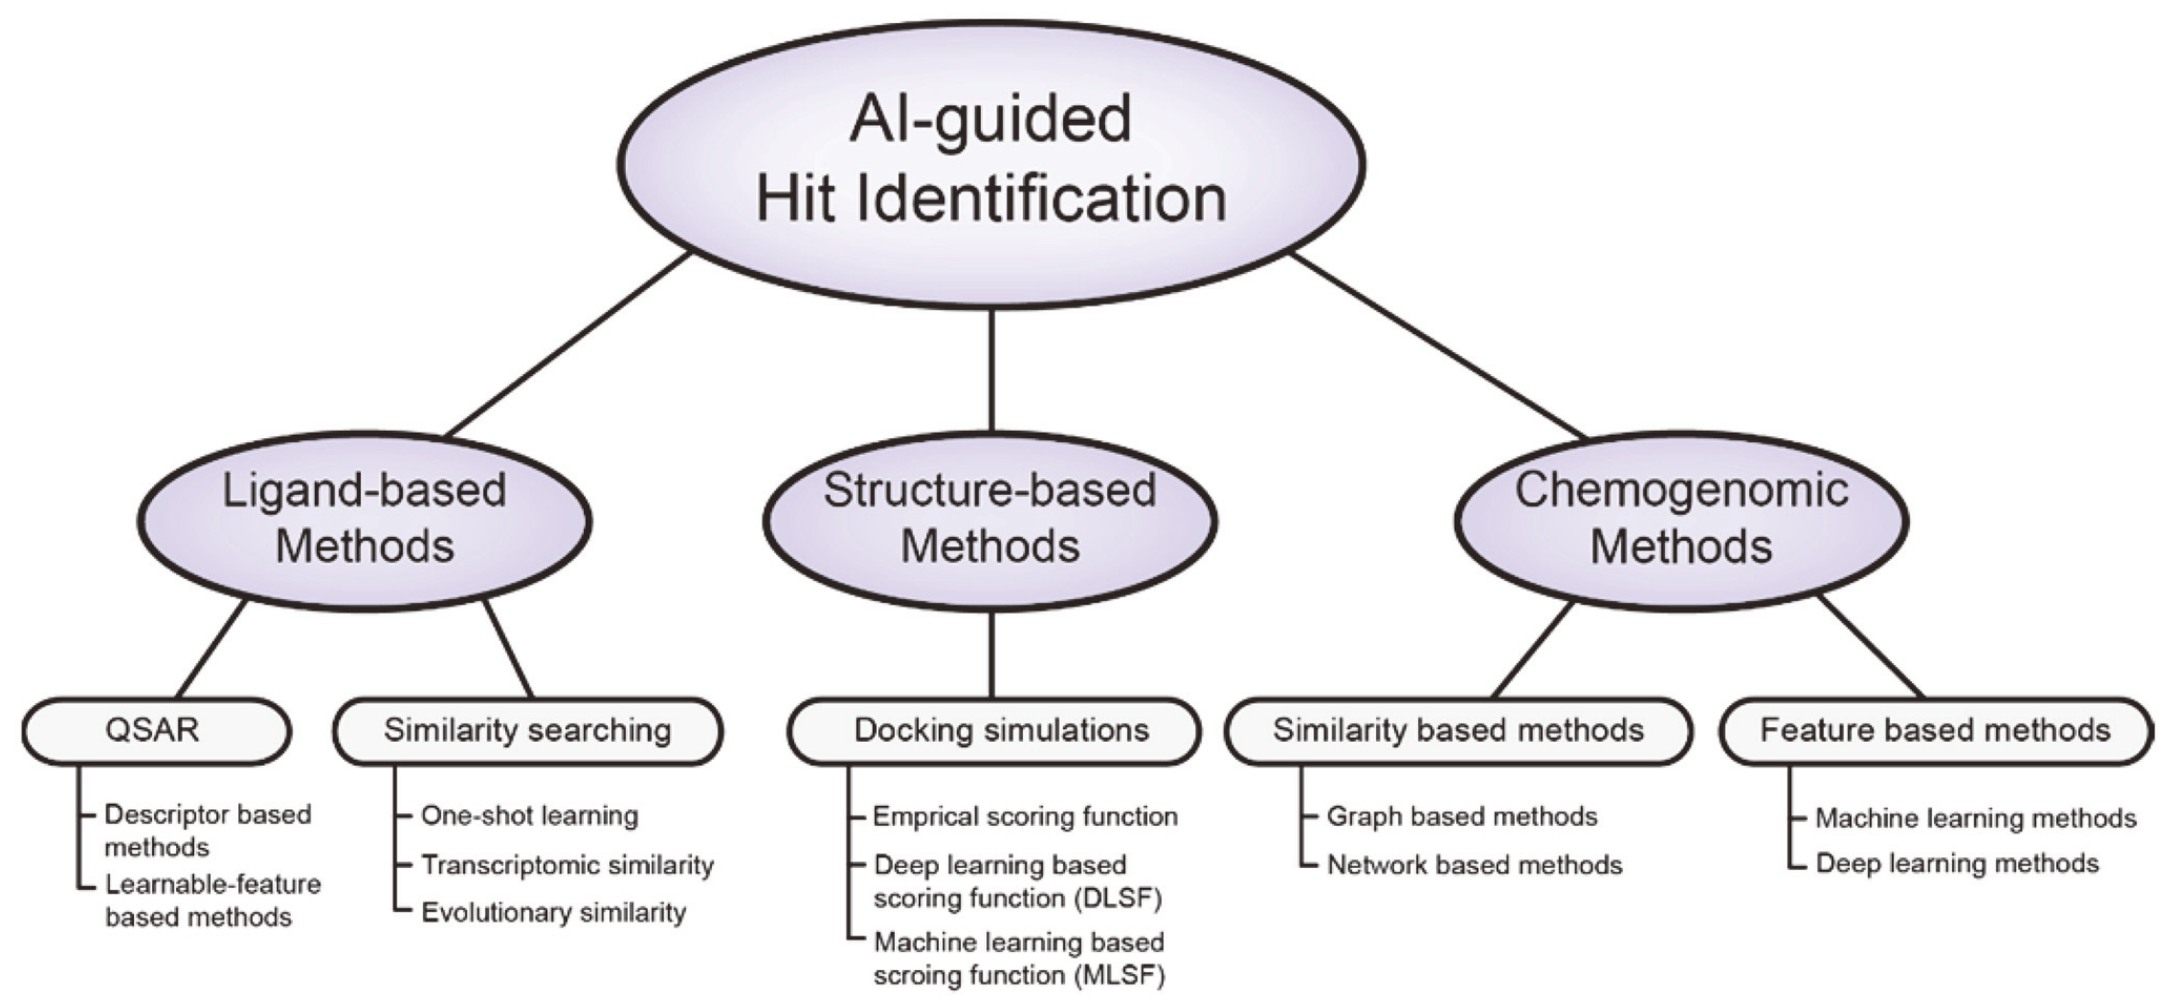
\includegraphics[width=0.9\textwidth]{drug_discovery_ai}    
    \caption{Drug discovery ML powered HIT identification methods overview \cite{kim_artificial_2020}}
    \label{fig:drug_discovery_ai}
\end{figure}

Datasets and task related to QSAR applications are the main bases for experiments of this work and further described in section \ref{sec:datasets}.

\subsubsection{Quantitative Structure-Activity Relationship}

One foundation of quantitative structure-activity relationship (QSAR) models is a study by Hansch et al.\cite{hansch_correlation_1962} in 1962 in which over 15 years the structure-activity relationship of growth regulators in plants have been analyzed finding out a suitable relationship which in the end turned out to be a dependency between the Hammett constant and hydrophobicity.  
Within QSAR applications the typical setup refers to a set of molecules for which a measurable biological property is known. Such a measurement usually refer to some potency value of a molecule having a corresponding effect and are typically originally measured in-vitro \cite{cherkasov_qsar_2014}. 
One widely used measurement is the half-maximum inhibitory concentration ($IC_{50}$). $IC_{50}$ describes the potential of an substance to inhibit a biological activity by 50\%. $IC_{50}$ is often given as $-log_{10}(IC_{50})$ in mol/L and referred to as $pIC_{50}$. Higher $pIC_{50}$ values therefore indicate a more potent inhibitor \cite{noauthor_ic50_2021}.
Formally defined a QSAR model describes the activity or target $a$ of a given compound or molecule $M$ in the form of a function $f$:

\begin{equation}
    a = f(M)
\end{equation}

Depending on the task or target $a$ such a QSAR model solves a regression (e.g. relating to the quantitative potency values) or as a classification problem (e.g. qualitative binary problem being active/inactive, toxic/non-toxic etc.) \cite{cherkasov_qsar_2014}. Given the nature of the problem, modeling QSAR using ML has shown great success and become a obvious choice in many cases \cite{ma_deep_2015}.

\subsubsection{Molecule Descriptors and Fingerprints} \label{sssec:molecule_descriptors_and_fingerprints}

One key component for in silico drug discovery and QSAR modeling is how molecules and components are represented for computational processing. For this common descriptors and molecule fingerprints are introduced:

\begin{itemize}
    \item \textbf{Simplified Molecular Input Line Entry Specification (SMILE)} - from theory point of view not a molecular descriptor or fingerprint but a common representation for molecules in a sequence of characters. Originally introduced in the 1980s \cite{weininger_smiles_1988} further development lead to the OpenSMILES standard in 2007. Their are many rules how to represent a molecule and described in the official specification \cite{noauthor_opensmiles_nodate}. An example for a SMILE representation of Aspirin is "O=C(C)Oc1ccccc1C(=O)O", this is also referred to as the SMILE string representation. 

    \item \textbf{0D descriptors} - do not account for structural information within a molecule. Examples are number of atoms, number of bonds or other atomic properties \cite{carracedo-reboredo_review_2021}

    \item \textbf{1D descriptors} - usually describe information from factions or part of a molecule. Based on chemical functional groups properties examples are number of primary carbons, number salts or cyanante containing etc. \cite{carracedo-reboredo_review_2021}.

    \item \textbf{2D descriptors} - are based on a 2D representation, usually in graph form, of a molecule. The structural topology is used like the adjacency and distance between atoms. Additionally topochemical information like properties of atoms (e.g. hybridization) can be incorporated \cite{carracedo-reboredo_review_2021}.

    \item \textbf{3D descriptor} - are using the 3D representation of a molecule, like distance of bonds or angels but also conformer of a molecule are considered. It is a more complex process and requires more computational resources \cite{carracedo-reboredo_review_2021}.

    \item \textbf{4D descriptor} - beside using the 3D representation also the interactions with other molecules in the 4th dimension can be considered \cite{carracedo-reboredo_review_2021}.

    \item \textbf{Extended Connectivity Fingerprints (ECFP)} - is a widely used molecule representation which results in a fixed size fingerprint of a particular molecule. Creating a ECFP representation is an iterative process:

    \begin{enumerate}
        \item Each atom within a molecule a 32 bit integer is assigned. The integer is determined based on the Daylight atomic invariant rule. This rule is invariant regarding the number an atom is assigned within a molecule and consists of six properties: Number of nearest-neighbors (non-hydrogen), number of bonds (non-hydrogen), atomic number, atomic mass, atomic charge, bond order ignoring (ignoring hydrogen bonds) and number of connected hydrogen. Optional the property of an atom being part(1) of a ring or not(0) is added as a seventh property \cite{sihag_beginners_2021}. Determining those 6 properties results in an array is formed which is hashed resulting in a single 32 bit integer for given atom. In the following figure \ref{fig:ecfp_sample1} for a sample molecule butyramide the individual atomic identifiers are presented.

        \begin{figure}[H]
            \centering
            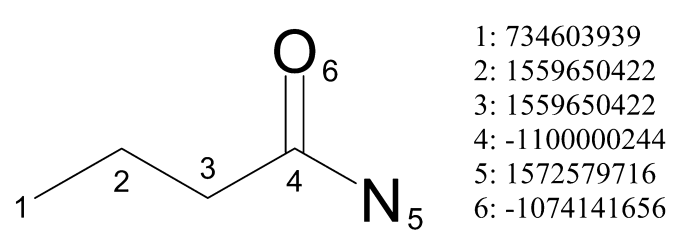
\includegraphics[width=0.7\textwidth]{ecfp_sample1}    
            \caption{Atom identifier for butyramide using Daylight atomic invariants rule \cite{rogers_extended-connectivity_2010}}
            \label{fig:ecfp_sample1}
        \end{figure}

        \item In the next step neighbor atom information are incorporated. For this an array is created starting with the center atom. For example considering atom 4 with identifier "-1100000244" in figure \ref{fig:ecfp_sample1}. All neighboring atoms with their integer identifiers are added including information about the bond type (1 single, 2 double, 3 triple and 4 for aromatic bonds) resulting in [1, -1100000244, 1, 1559650422, 1, 1572579716, 2, -1074141656]. This array again is hashed and getting a new integer identifier “-1708545601” which is added to the overall list of identifiers. After the first iteration this results for the mentioned example in the list [734603939, 1559650422, 1559650422, -1100000244, 1572579716, -1074141656, 863188371, -1793471910, -1789102870,  1708545601, -932108170, 2099970318] \cite{rogers_extended-connectivity_2010}.
        
        This process can be repeated multiple times resulting in a larger radius around an atom considered, and is a hyperparameter for the ECFP molecule representation method.

        \item To get a fixed size numerical representation, often desired and used as input to a corresponding QSAR model, a modulo operator (remainder of a division) is applied onto the individual identifiers. Using 1024 for the value of the modulo operator this would result in $[675, 118, 118, 12, 388, 552, 403, 602, 234, 447, 118, 270]$ for mentioned identifiers of butyramide. The fixed size representation is achieved by creating a binary vector of length 1024 and assigned 1 for all indices found in the modulo operator. Depending on the value of the modulo operator this lead to a high sparsity in the representation (if the value is large) or more bit collisions. Bit collisions appear if multiple identifiers end up assigning 1 to the same index. In the above mentioned this happened for the index $118$ which was assigned thrice. 
        The process of creating a fixed size representation is also referred to as folding \cite{rogers_extended-connectivity_2010}.
    \end{enumerate}

    \item \textbf{Molecular ACCess System (MACCS keys)} - refer to set of pattern in a molecule which must be present to define a fixed length binary vector. The set consists of 166 public available patterns resulting in a fixed size binary vector of length 166 representing a molecule. MACCS keys were original developed by MDL Information Systems and include 960 patterns but only a set of 166 patterns were made publicly available \cite{durant_reoptimization_2002}

    Those patterns are described in the form of SMILE arbitrary target specification (SMARTS) pattern. As the name suggests it is related to SMILE representation and allows flexibility and precise substructure specification including wildcard matching. For the detailed specification refer to official specification \cite{noauthor_daylight_nodate}.

\end{itemize}

\newpage

\end{document}